\chapter{Implementacja systemu}
\label{cha:implementacja}

Celem omawianego rozdziału jest przedstawienie implementacji proponowanego w Rozdziale \ref{cha:propozycja-systemu} systemu automatyki domowej. Niniejsza część została podzielona na dwie sekcje. W pierwszej sekcji zaprezentowana zostanie stworzona na potrzeby projektu sieć Thread. Kolejny fragment poświęcony jest warstwie aplikacji, technologiom wykorzystanym przy wdrażaniu komponentów oraz zasadzie działania systemu.

Projekt aplikacji systemu znajduje się w stworzonym przez autora pracy repozytorium \cite{project-repo}.

\section{Sieć Thread}

    \subsection{Założenia}
    \label{sec:thread-network-assumptions}
    
        Do stworzenia sieci Thread wykorzystano 5 urządzeń Nordic Semiconductor nRF52833 oraz Laptop Dell G3 15 z procesorem Intel Core i7 9. generacji, z systemem operacyjnym Microsoft Windows 11. Przed procesem implementacji sieci Thread, dokonano następujących założeń:
        \begin{itemize}
            \item Jedna platforma nRF52833 wraz z laptopem Dell zostaną wykorzystane do pełnienia roli Rutera brzegowego.
            \item Dwa urządzenia nRF52833 zostaną skonfigurowane do typu MTD oraz będą stanowiły urządzenia końcowe, MED oraz SED, które w warstwie aplikacji będą pełniły rolę profili HEATER oraz DIMMER.
            \item Dwa urządzenia nRF52833 zostaną skonfigurowane do typu FTD. Zostaną one wprowadzone do sieci, aby wprowadzić nadmiarowość i pozwolić Liderowi Thread na dostosowanie topologii do aktualnych potrzeb i wymagań sieci.
        \end{itemize}

        Na Rysunku \ref{fig:thread-topology} przedstawiono przykładową topologię sieci Thread, złożoną z wyszczególnionych powyżej urządzeń.

        \begin{figure}[H]
            \centering
            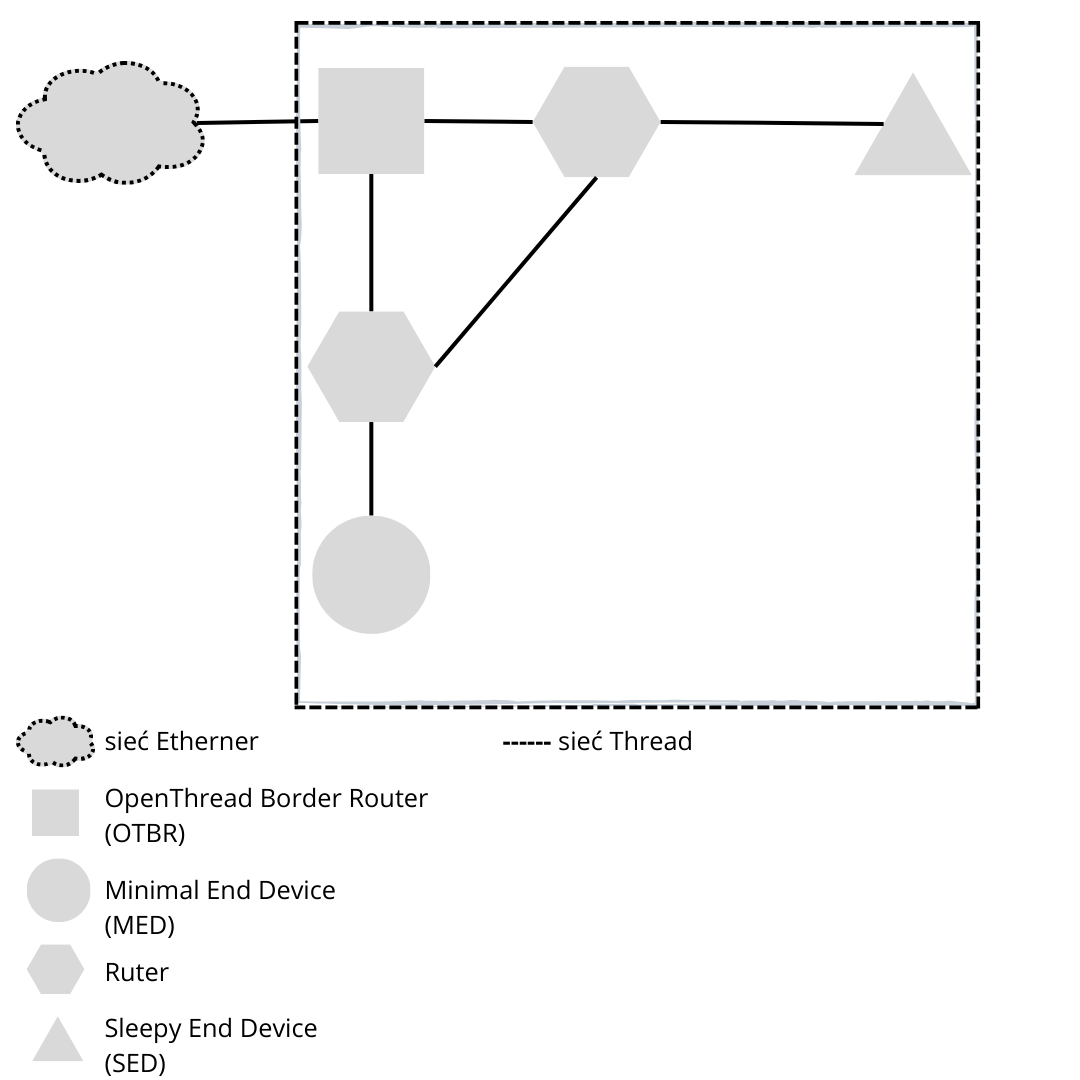
\includegraphics[width=0.8\linewidth]{graphics/thread-topology.png}
            \caption{Przykładowa topologia sieci Thread złożona z urządzeń wymienionych w założeniach w Sekcji \ref{sec:thread-network-assumptions}.}
            \label{fig:thread-topology}
        \end{figure}

    \subsection{Ruter Brzegowy}

        W celu zapewnienia komunikacji przyszłej sieci Thread z zewnętrzną siecią Ethernet, w pierwszej kolejności przystąpiono do uruchomienia oraz konfiguracji Rutera brzegowego, wykorzystując implementację OTBR. 
        
        Aplikacja OTBR jest dedykowana dla systemów operacyjnych Linux oraz do poprawnego działania wymaga nawiązania komunikacji zarówno z interfejsem sieci Thread, jak również z interfejsem sieci zewnętrznej. Z tego powodu, w początkowym kroku skonfigurowano platformę Linux, jako maszynę wirtualną z dystrybucją Ubuntu, tak aby zapewnić komunikację sieciową oraz komunikację portów szeregowych między urządzeniem gościa (maszyną wirtualną) a gospodarza (ang. \textit{Host}) (Laptop Dell). Kolejno skonfigurowano środowisko deweloperskie, instalując niezbędne narzędzia deweloperskie, takie jak system kontroli wersji Git, IDE (ang. Integrated Development Environment) itp.. 
        
        Po weryfikacji poprawności działania maszyny wirtualnej, kontynuowano proces uruchomienia OTBR, wykorzystując instrukcję zamieszczoną na oficjalnej stronie projektu OpenThread \cite{otbr-docker}. Zaprogramowano jedno z urządzeń nRF52833 aplikacją RCP (ang. Radio Co-Processor), używając dostarczoną przez OpenThread implementację \cite{otbr-rcp-app}. Podłączona zaprogramowaną platformę do portu szeregowego urządzenia gościa, a następnie sprawdzono poprawność komunikacji między maszyną wirtualną a urządzeniem pracującym jako RCP. Ostatecznie uruchomiono kontener Docker, zawierający aplikację OTBR. Upewniwszy się o poprawnym działaniu Rutera brzegowego, rozpoczęto tworzenie sieci Thread.
    
        Do konfiguracji sieci wykorzystano interfejs graficzny OTBR Web GUI, będący serwisem zapewnionym w ramach aplikacji OTBR. Zrzut ekrany przedstawiającego wymieniony interfejs graficzny, zaprezentowano na Rysunku \ref{fig:otbr-web-gui}.
        
        \begin{figure}[H]
            \centering
            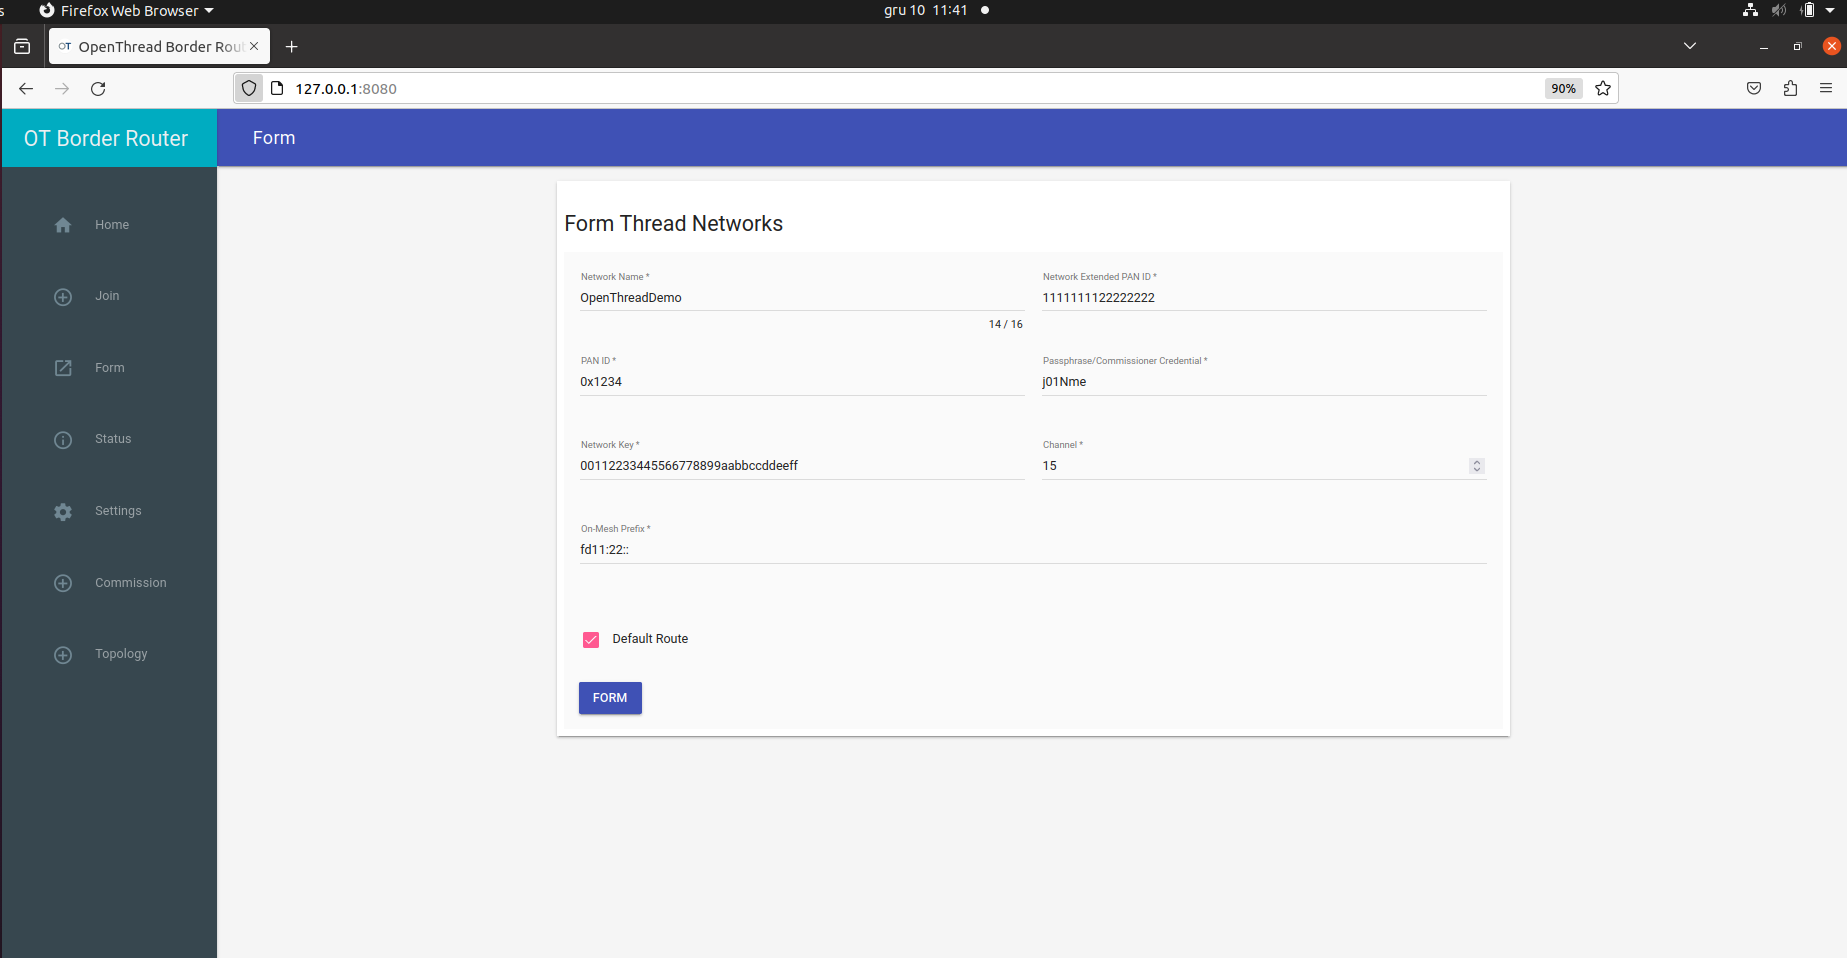
\includegraphics[width=0.8\linewidth]{graphics/screenshots/OTBR-web-gui.png}
            \caption{Zrzut ekranu interfejsu OTBR GUI z oknem do tworzenia sieci Thread.}
            \label{fig:otbr-web-gui}
        \end{figure}
        
        Wartości parametrów koniecznych do stworzenia sieci Thread, które opisano w Podsekcji \ref{subsec:network-forming}, przedstawiono w Tabeli \ref{tab:network-parameters}.
    
            \begin{table}[H]
            \centering
            \caption{Parametry sieci Thread.}
            \begin{tabular}{|l|l|}
                \hline
                \rowcolor{gray!20}
                 \multicolumn{1}{|c|}{\textbf{Nazwa parametru}} & \multicolumn{1}{|c|}{\textbf{Wartość}}  \\
                 \hline
                 Network Name & pawel\_network \\
                 \hline
                 PAN ID & 0x0457 \\
                 \hline
                 Network Key & 00112233445566778899aabbccddeeff \\
                 \hline
                 Extended PAN ID & fb020000abcd0000 \\
                 \hline
                 Commissioning Credential & J01NME \\
                 \hline
                 Channel & 13 \\ 
                 \hline
                 Mesh-Local Prefix & fd11:22:: \\
                 \hline
            \end{tabular}
            \label{tab:network-parameters}
        \end{table}
    
        Po zatwierdzeniu parametrów, a w konsekwencji utworzeniu sieci Thread, skonfigurowano Ruter brzegowy, aby pracował jako Commissioner w procesie przedstawionym w Podsekcji \ref{subsec:commissioning}. W tym celu wykorzystano OpenThread CLI \cite{otbr-cli}. Narzędzie to pozwala na konfigurację urządzeń sieci Thread, w których wdrożono OpenThread. Na Rysunku \ref{fig:ctl-commissioner} przedstawiono wprowadzone w konsolę OpenThread CLI komendy, konfigurujące rolę Commissioner w Ruterze brzegowym oraz pozwalające na dołączenie do sieci wszystkim urządzeniom posiadającym Commissioning Credential o wartości \textit{J01NME}.
    
            \begin{figure}[H]
            \centering
            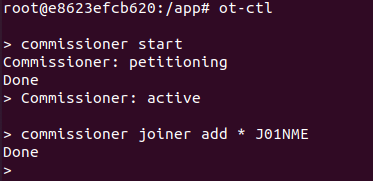
\includegraphics[width=0.8\linewidth]{graphics/screenshots/ot-ctl-commissioning.png}
            \caption{Zrzut ekranu konsoli OpenThread CLI, przedstawiający konfigurację roli Commissioner.}
            \label{fig:ctl-commissioner}
        \end{figure}
    
        Tak skonfigurowane urządzenie jest w pełni funkcjonalnym Ruterem brzegowym, pracującym w roli Commissioner.

    \subsection{Urządzenia MTD oraz FTD}
    \label{subsubsec:mtd-ftd-devices-implementation}

    Aplikację dla 4 pozostałych urządzeń nRF52833 stworzono w języku C z wykorzystaniem nRF Connect SDK oraz środowiska programistycznego nRF Connect IDE. W plikach konfiguracyjnych projektów skonfigurowano odpowiednio stos protokołu i niezbędne funkcjonalności Thread, system logowanie, GPIO (ang. \textit{general-purpose input/output}). Kolejno wybrano tryb MTD dla 2 urządzeń, natomiast dla pozostałych FTD. Zadbano, aby każde z urządzeń po włączeniu zasilania automatycznie dołączały do sieci o podanym Commissioning Credential. 

    Dodatkowo, w urządzeniach MTD uwzględniono możliwość przejścia w tryb energooszczędny, poprzez naciśnięci przycisku, w wyniku czego ED zmienia pełniącą rolę z MED na SED oraz obniża zużycie energii w wyniku ograniczenia zużycia pamięci RAM.

    Na potrzeby procesu rozwoju oprogramowania, wzbogacono wszystkie 4 platformy, o sygnalizację stanu urządzenia Thread przy pomocy LED (ang. \textit{ang. light-emitting diode}).
    
\section{Warstwa Aplikacji}

    Do wymiany informacji podczas komunikacji klient-serwer między urządzeniami końcowymi w sieci Thread a System Controllerem, wykorzystano protokół warstwy aplikacji Constrained Application. CoAP jest protokołem opartym o REST API (ang. \textit{Representational State Transfer Application Programming Interface}), który nawiązuje połączenie z wykorzystaniem wspieranego przez stos Thread protokołu UDP.

    \subsection{Implementacja komponentów systemy}

        Obecna sekcja ma za zadanie przybliżyć szczegóły implementacji poszczególnych komponentów wymienionych w Rozdziale \ref{cha:propozycja-systemu}.

        \subsubsection{Baza danych}
            Przez wzgląd na mały rozmiar, pełne wsparcie funkcjonalności SQL (ang. \textit{Structured Query Language}) oraz możliwość przechowywania bazy danych w pojedynczym pliku, jako silnik, wykorzystywanej w projekcie systemu, bazy danych wybrano SQLite. \cite{sqlite}.

            Stworzony na potrzeby systemu zestaw tabel bazy danych przedstawiono na Rysunku \ref{fig:db-diagram}.

            \begin{figure}[H]
                \centering
                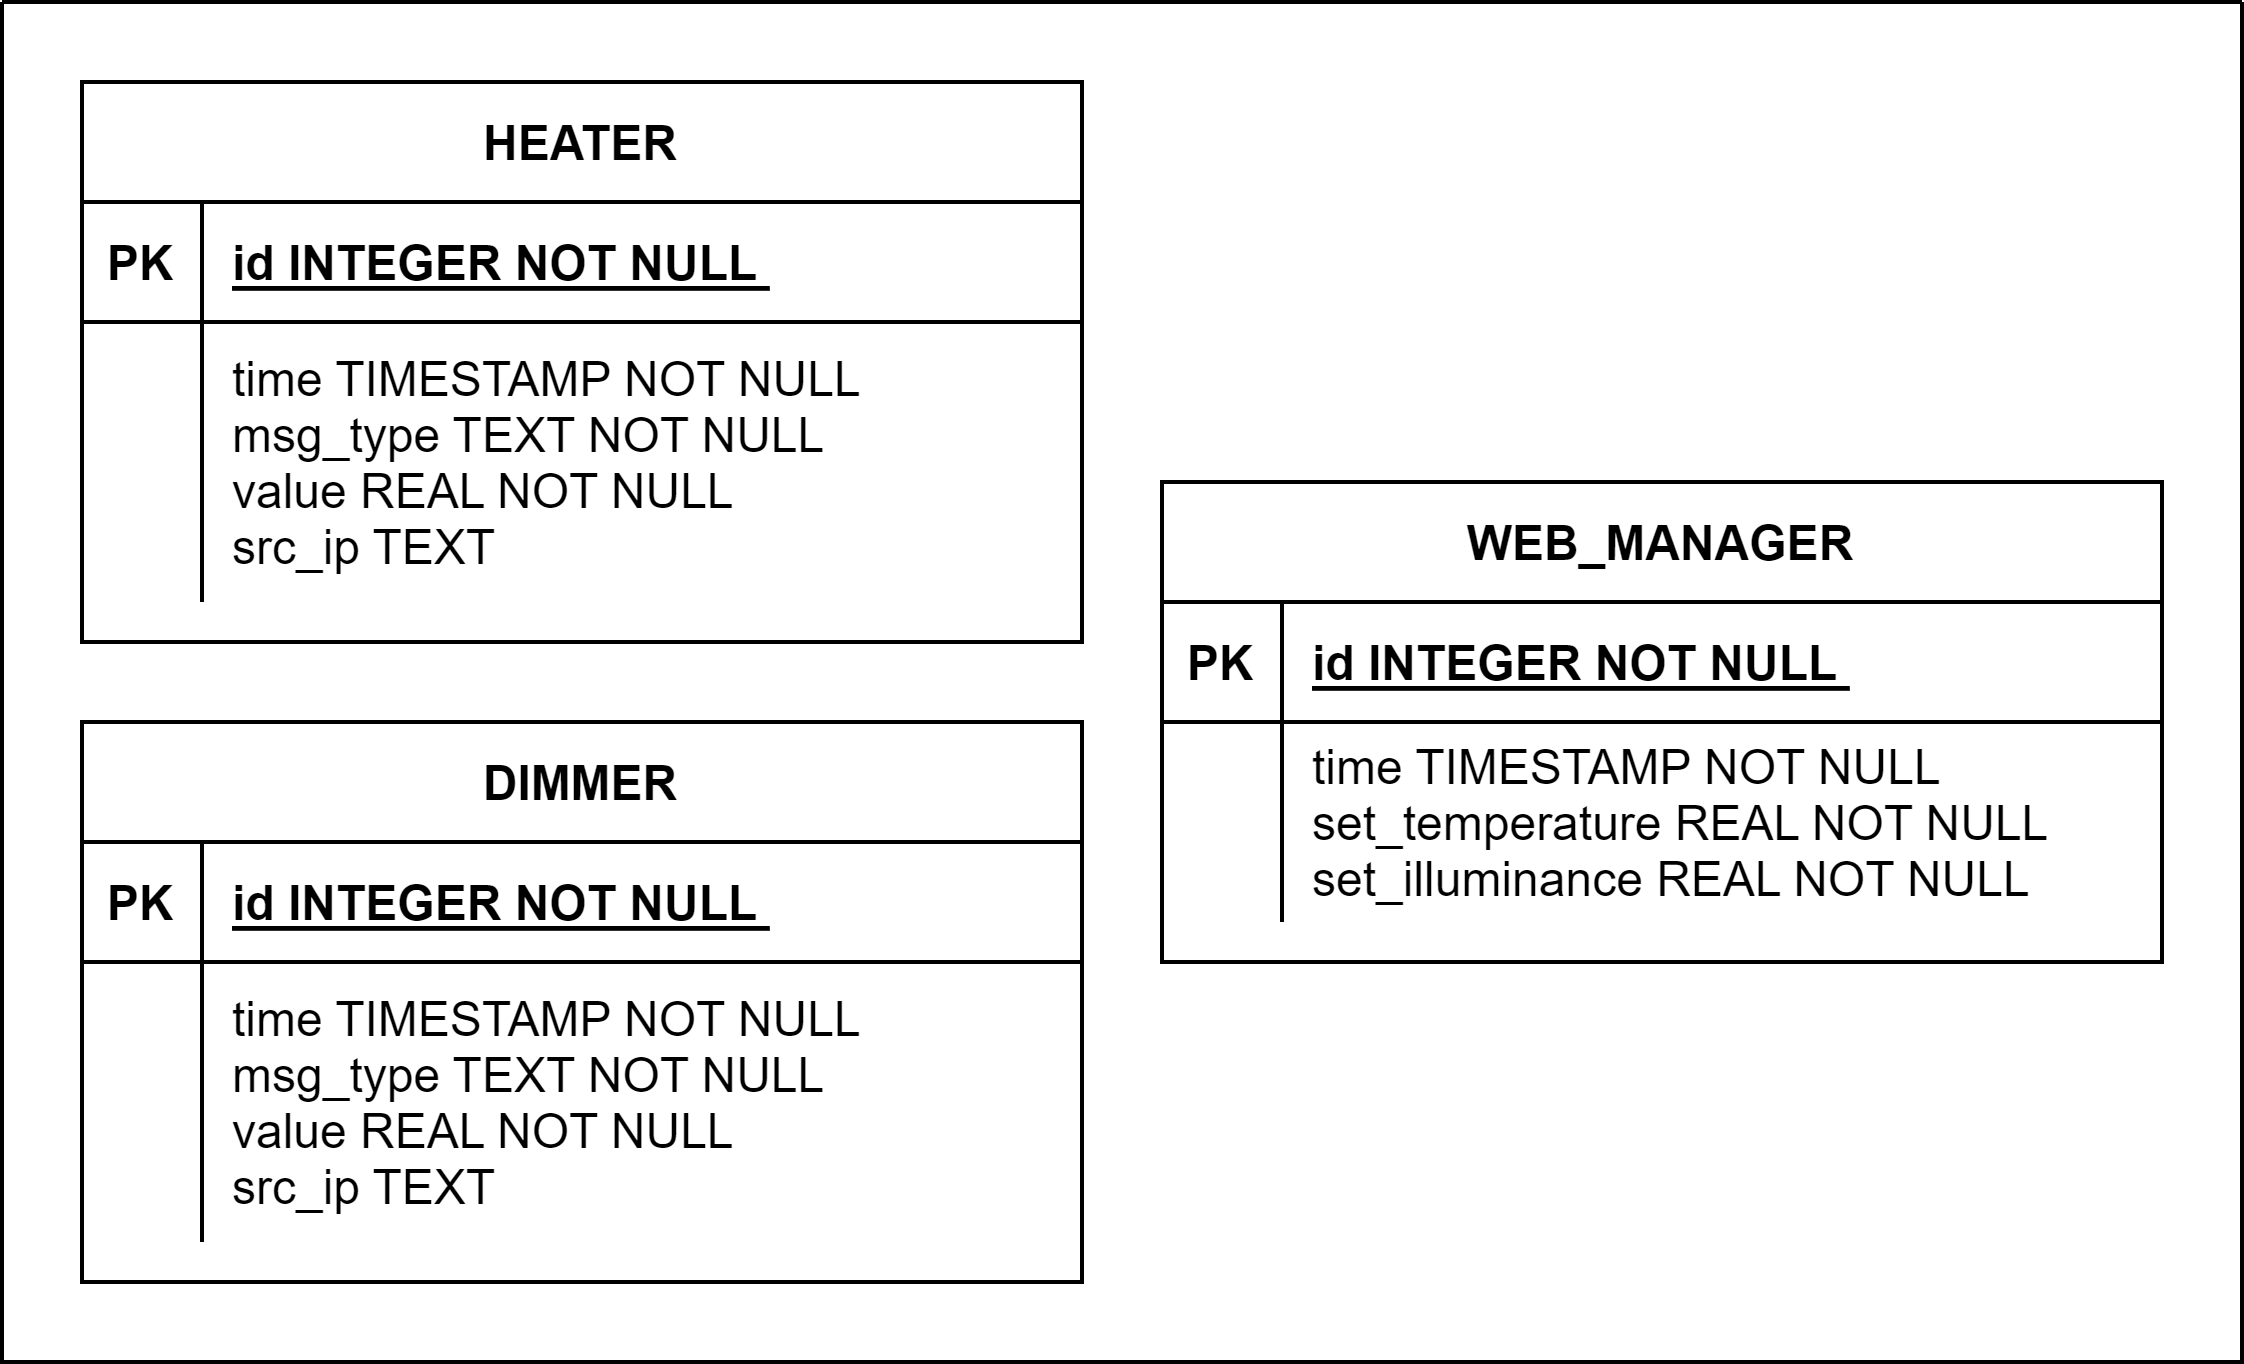
\includegraphics[width=0.8\linewidth]{graphics/db_diagram.png}
                \caption{Schemat tabel baz danych systemu.}
                \label{fig:db-diagram}
            \end{figure}
    
        \subsubsection{System Controller}
    
            System Controller został wdrożony jako aplikacja w języku Python, przeznaczona dla urządzeń z systemem operacyjnym Linux.
            System Controller odbiera żądania oraz wysyła odpowiedzi CoAP z wykorzystaniem dostarczonego przez bibliotekę aiocoap API \cite{aiocoap}. URI (ang. \textit{Uniform Resource Identifier}) zdefiniowanych zasobów serwera oraz ich funkcje, zdefiniowano w Tabeli \ref{tab:resurces}.
            
            Zarządzanie bazą danych SQLite odbywa się z użyciem wbudowanych w język Python bibliotek \textit{sqlite3} oraz \textit{aiosqlite}.

            \begin{table}[H]
                \centering
                \caption{Zasoby serwera CoAP.}
                \begin{tabular}{|l|l|l|}
                     \hline
                     \rowcolor{gray!20}
                     \multicolumn{1}{|c|}{Zasób} & \multicolumn{1}{c|}{Typ zapytań} & \multicolumn{1}{c|}{Funkcja} \\
                     \hline
                     temperature & GET, PUT & Przechowuje wartość aktualnej temperatury środowiska.\\
                     \hline
                     illuminance & GET, PUT & Przechowuje wartość aktualnego natężenia oświetlenia środowiska.\\
                     \hline
                     heater\_regulation & GET & Zwraca wartość parametru regulacji dla układu HEATER.\\
                     \hline
                     dimmer\_regulation & GET & Zwraca wartość parametru regulacji dla układu DIMMER.\\
                     \hline
                \end{tabular}
                \label{tab:resurces}
            \end{table}
    
        \subsubsection{HEATER oraz DIMMER}

            Platformy nRF52833 pracujące jako MTD, w których skonfigurowano stos Thread, jak opisano w Podsekcji \ref{subsubsec:mtd-ftd-devices-implementation}, wzbogacono o warstwę aplikacji. Urządzenia Końcowe symulują zachowanie zdefiniowanych w Sekcji \ref{sec:system-clients} profili HEATER oraz DIMMER. Wysyłanie zapytań oraz odbieranie odpowiedzi CoAP zaimplementowane jest z wykorzystaniem API dostarczonego przez nRF Connect SDK oraz OpenThread.
        
        \subsubsection{Web GUI}

            Interfejs użytkownika Web GUI stanowi aplikacja w języku Python, którą stworzono z użyciem następujących technologii webowych:
            \begin{itemize}
                \item mikro-frameworku Flask \cite{flask},
                \item CSS (ang. \textit{Cascading Style Sheets}),
                \item HTML (ang. \textit{HyperText Markup Language}).
            \end{itemize}
            Aplikacja komunikuje się bezpośrednio z bazą danych, wykorzystując bibliotekę sqlite3.

            \begin{figure}[H]
                \centering
                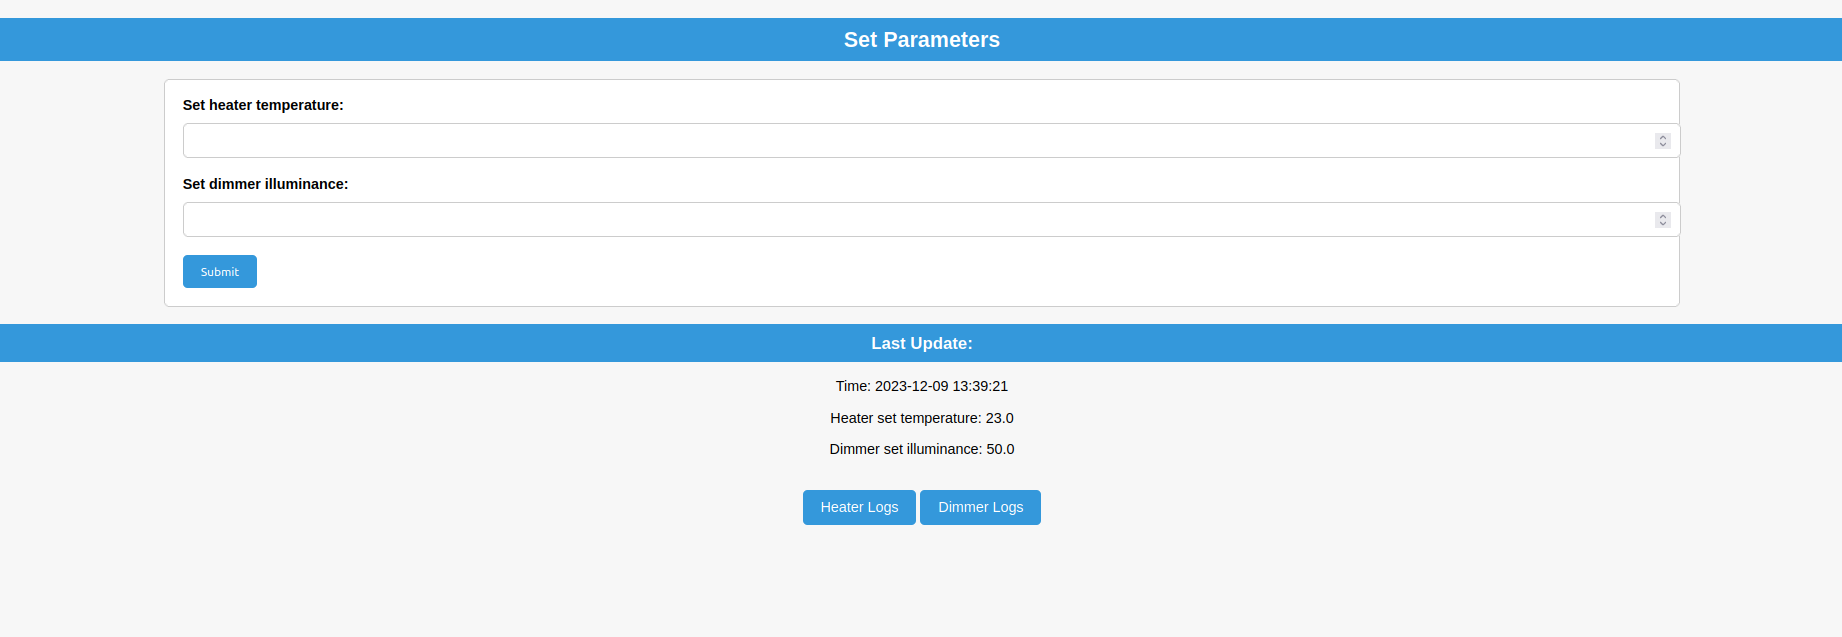
\includegraphics[width=0.8\linewidth]{graphics/screenshots/web-gui-set-parameters.png}
                \caption{Zrzut ekranu przedstawiający panel Web GUI przeznaczony do ustalania parametrów systemu.}
                \label{fig:web-gui-set-parameters}
            \end{figure}

            \begin{figure}[H]
                \centering
                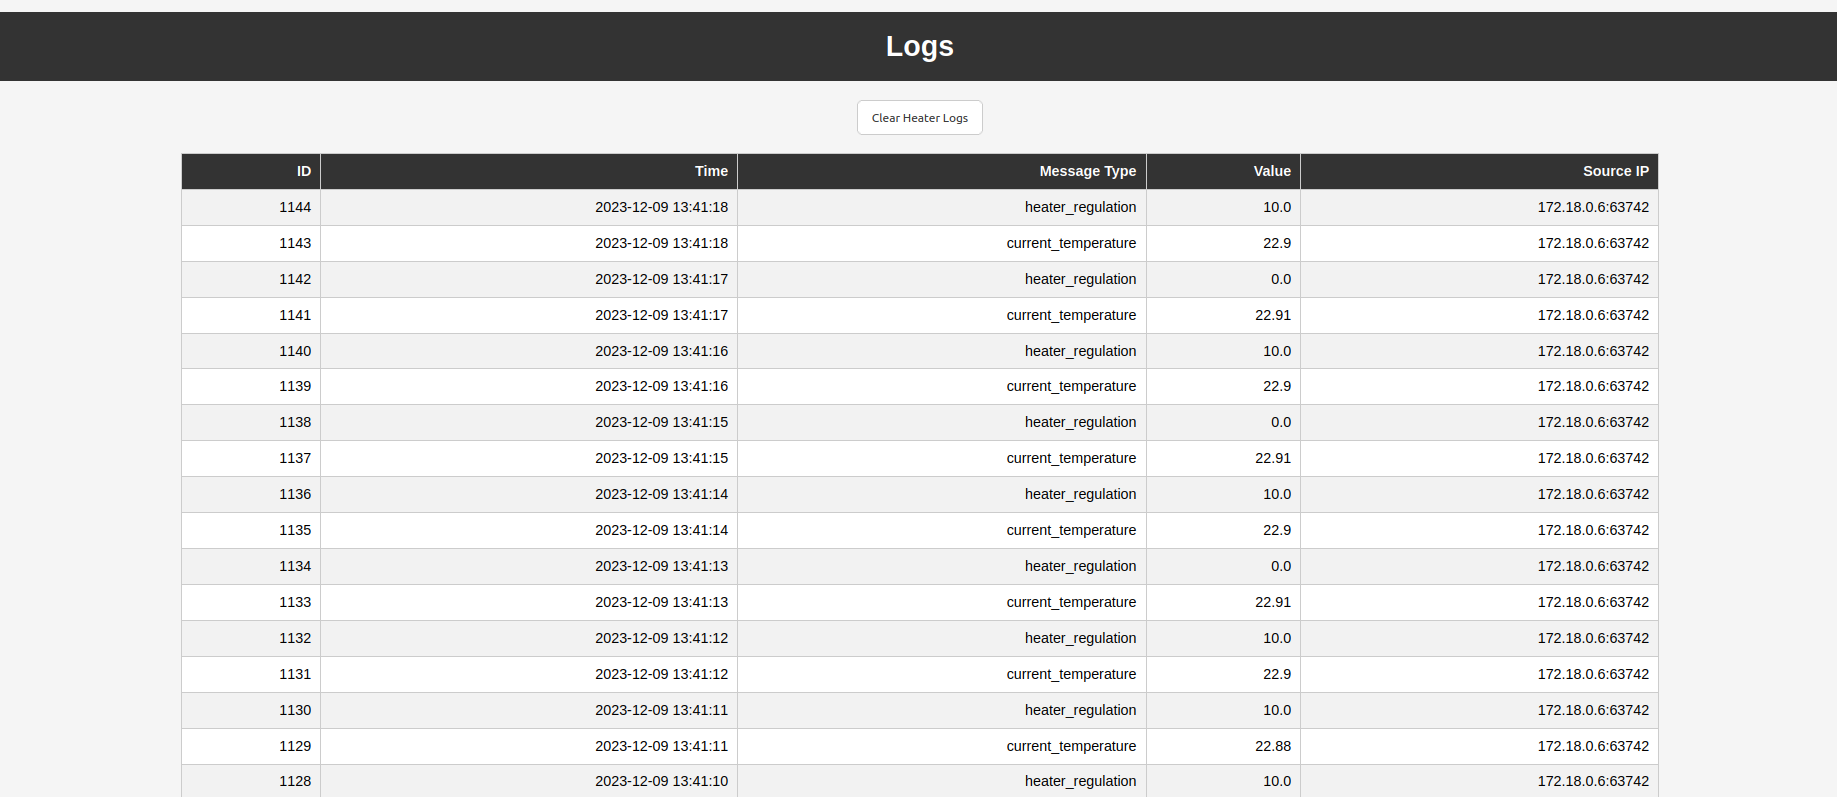
\includegraphics[width=0.8\linewidth]{graphics/screenshots/web-gui-logs.png}
                \caption{Zrzut ekranu przedstawiający panel Web GUI przeznaczony do obserwacji logów systemu.}
                \label{fig:web-gui-logs}
            \end{figure}

    \subsection{Zasada działania}

    Celem niniejszej Podsekcji jest opisanie zasady działania wdrożonego systemu automatyki domowej, poprzez przegląd logiki aplikacji oraz przepływu informacji między komponentami.
    
    Zachowanie systemu można podzielić na 3 fazy:
    \begin{itemize}
        \item Fazę ustalania parametrów systemu - użytkownik nadaje systemowi stan, do którego mają dążyć układy regulacyjne.
        \item Fazę pomiarów - układ pomiarowy przesyła aktualny stan parametru System Controllerowi
        \item Fazę regulacji - układ regulacji odpytuje System Controller o nową wartość parametru mocy w celu utrzymania parametrów środowiska dążących do zadanego przez użytkownika stanu.
    \end{itemize}

        \subsubsection{Ustalanie parametrów systemu}

            Na Rysunku \ref{fig:seq-user-webgui-db} zilustrowano przepływ wiadomości między komponentami systemu w fazie ustalania parametrów systemu.

            \begin{figure}[H]
                \centering
                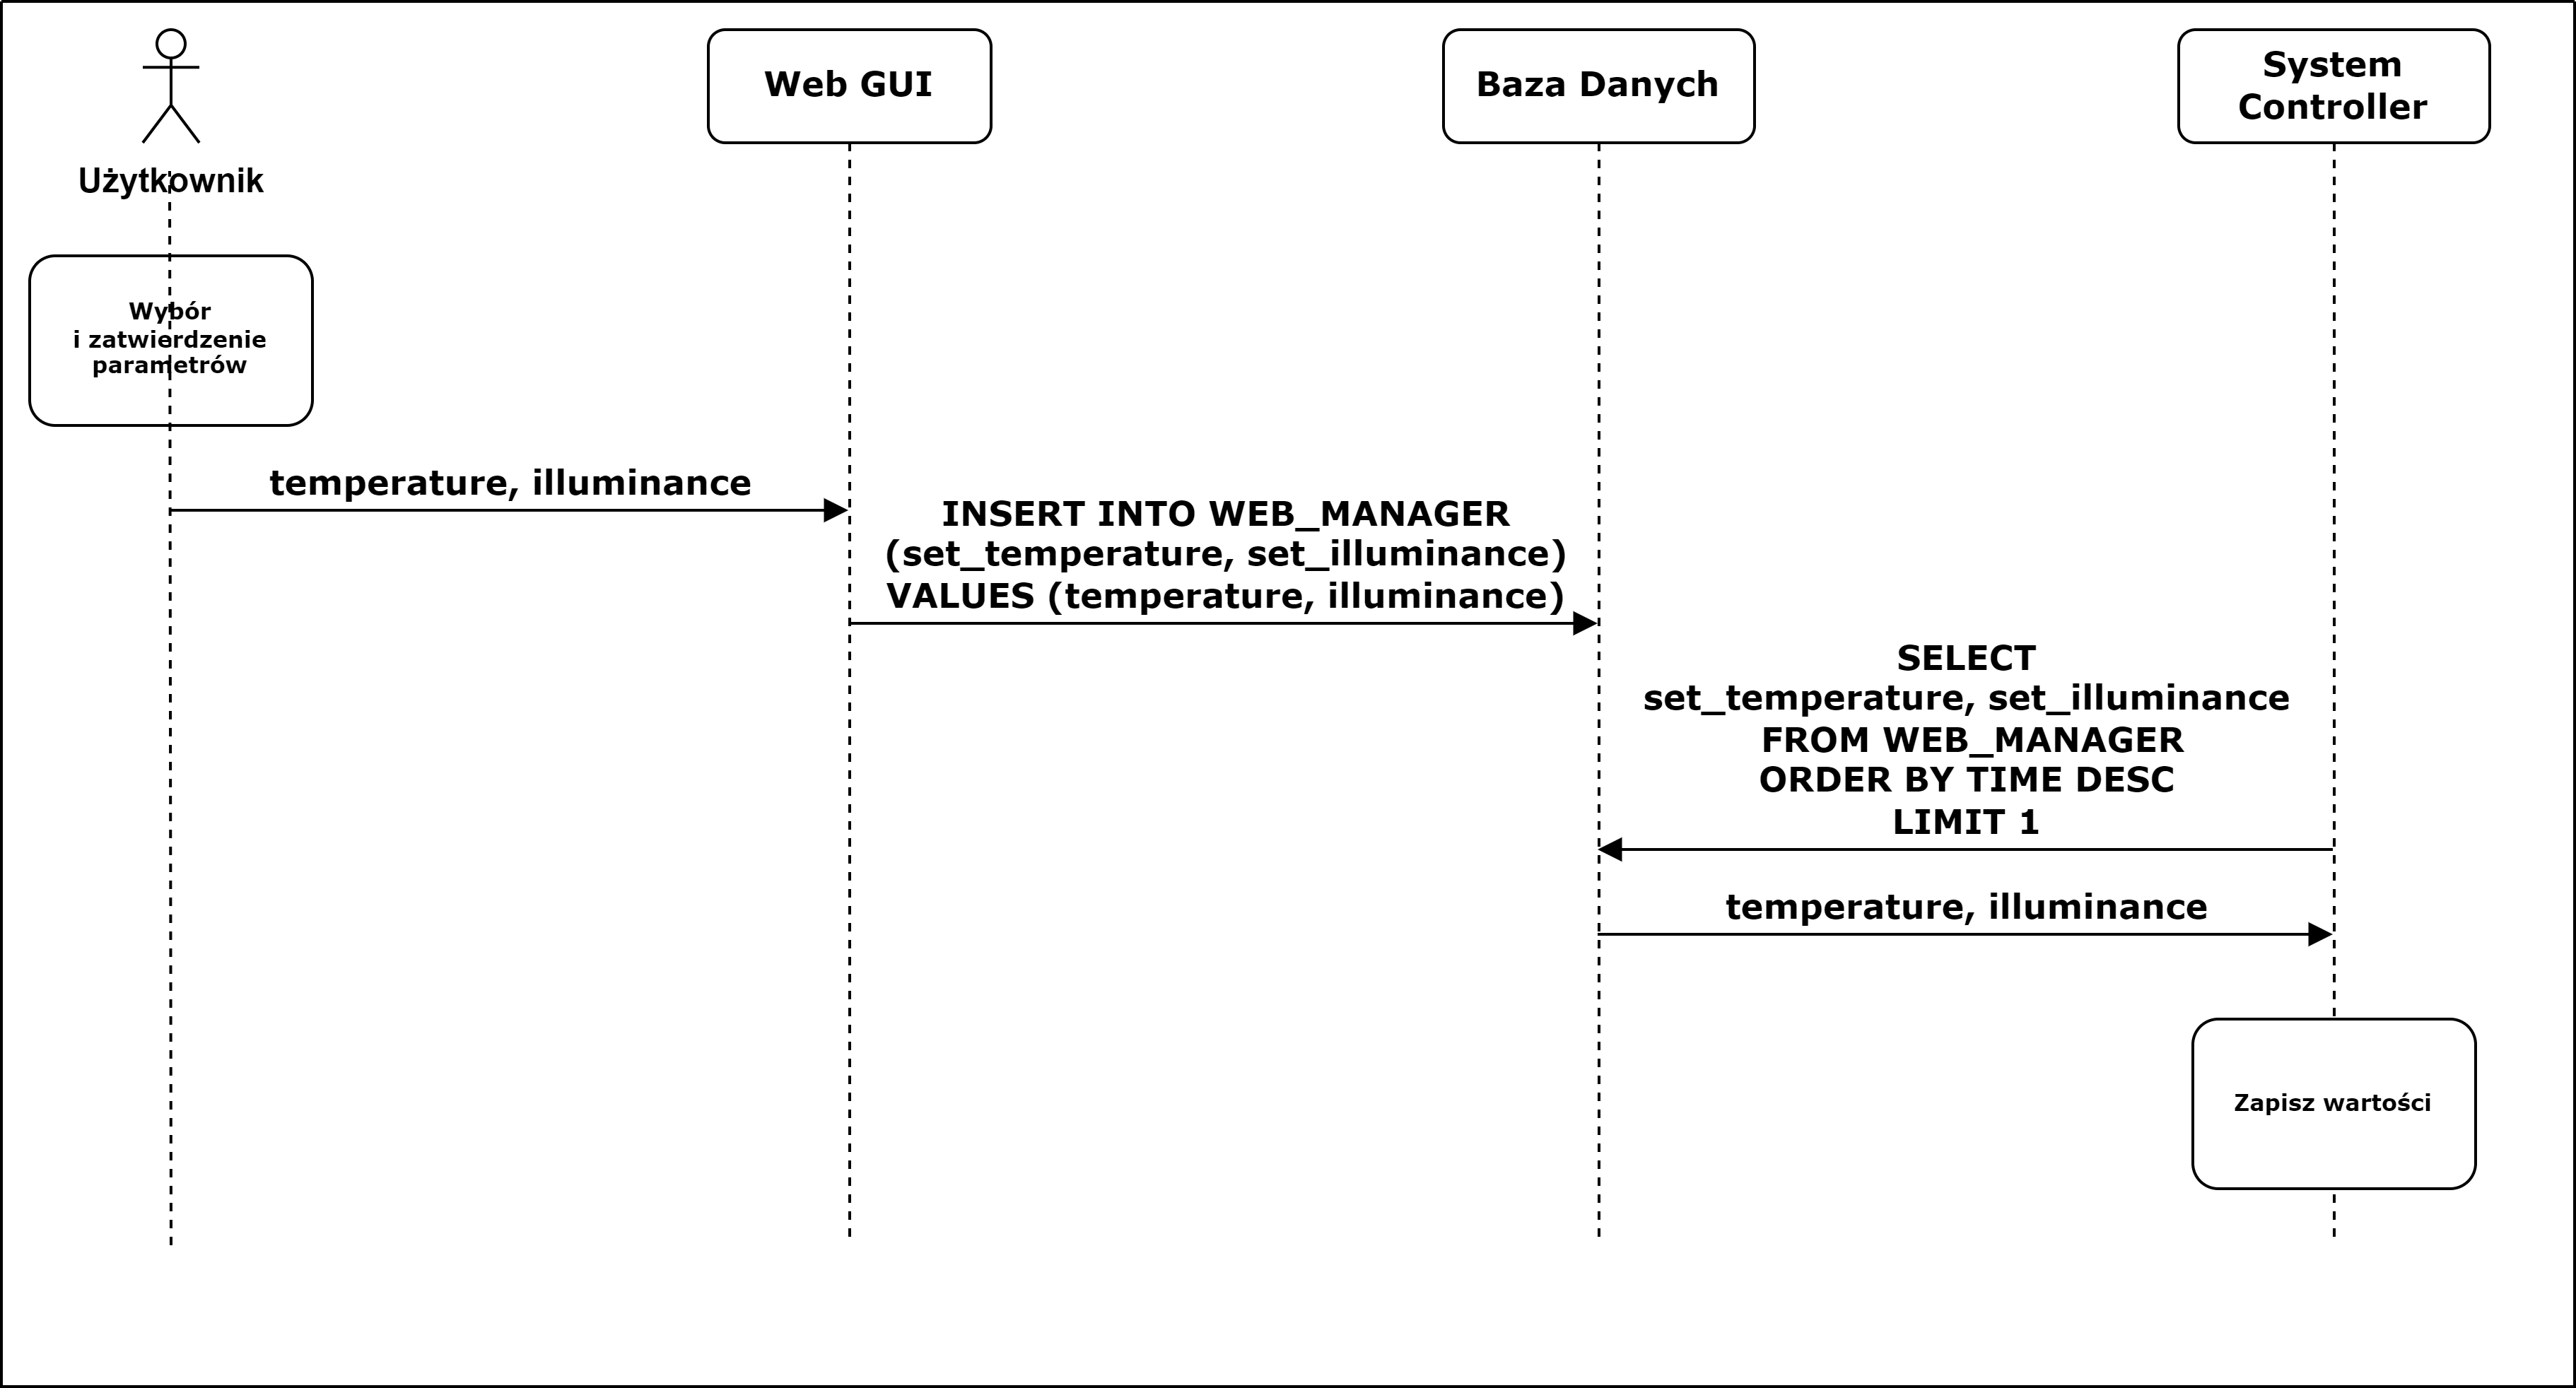
\includegraphics[width=0.8\linewidth]{graphics/sequence-diagrams/user-webgui-db-diagram.png}
                \caption{Diagram sekwencji ustawiania parametrów systemu.}
                \label{fig:seq-user-webgui-db}
            \end{figure}

            Kolejnymi krokami procedury są:
            \begin{enumerate}
                \item Użytkownik korzystający z panelu Web GUI, służącego do ustawiania parametrów system, zobrazowanym na Rysunku \ref{fig:web-gui-set-parameters}, podaje i zatwierdza wartości.
                \item Wprowadzone wartości \textit{temperature} oraz \textit{illuminance} wstawiane są do tabeli WEB\_MANAGER Bazy Danych.
            \end{enumerate}

        \subsubsection{Pomiar}

            Na Rysunku \ref{fig:seq-heater-measure} zilustrowano przepływ wiadomości między komponentami systemu w fazie pomiaru temperatury.

            \begin{figure}[H]
                \centering
                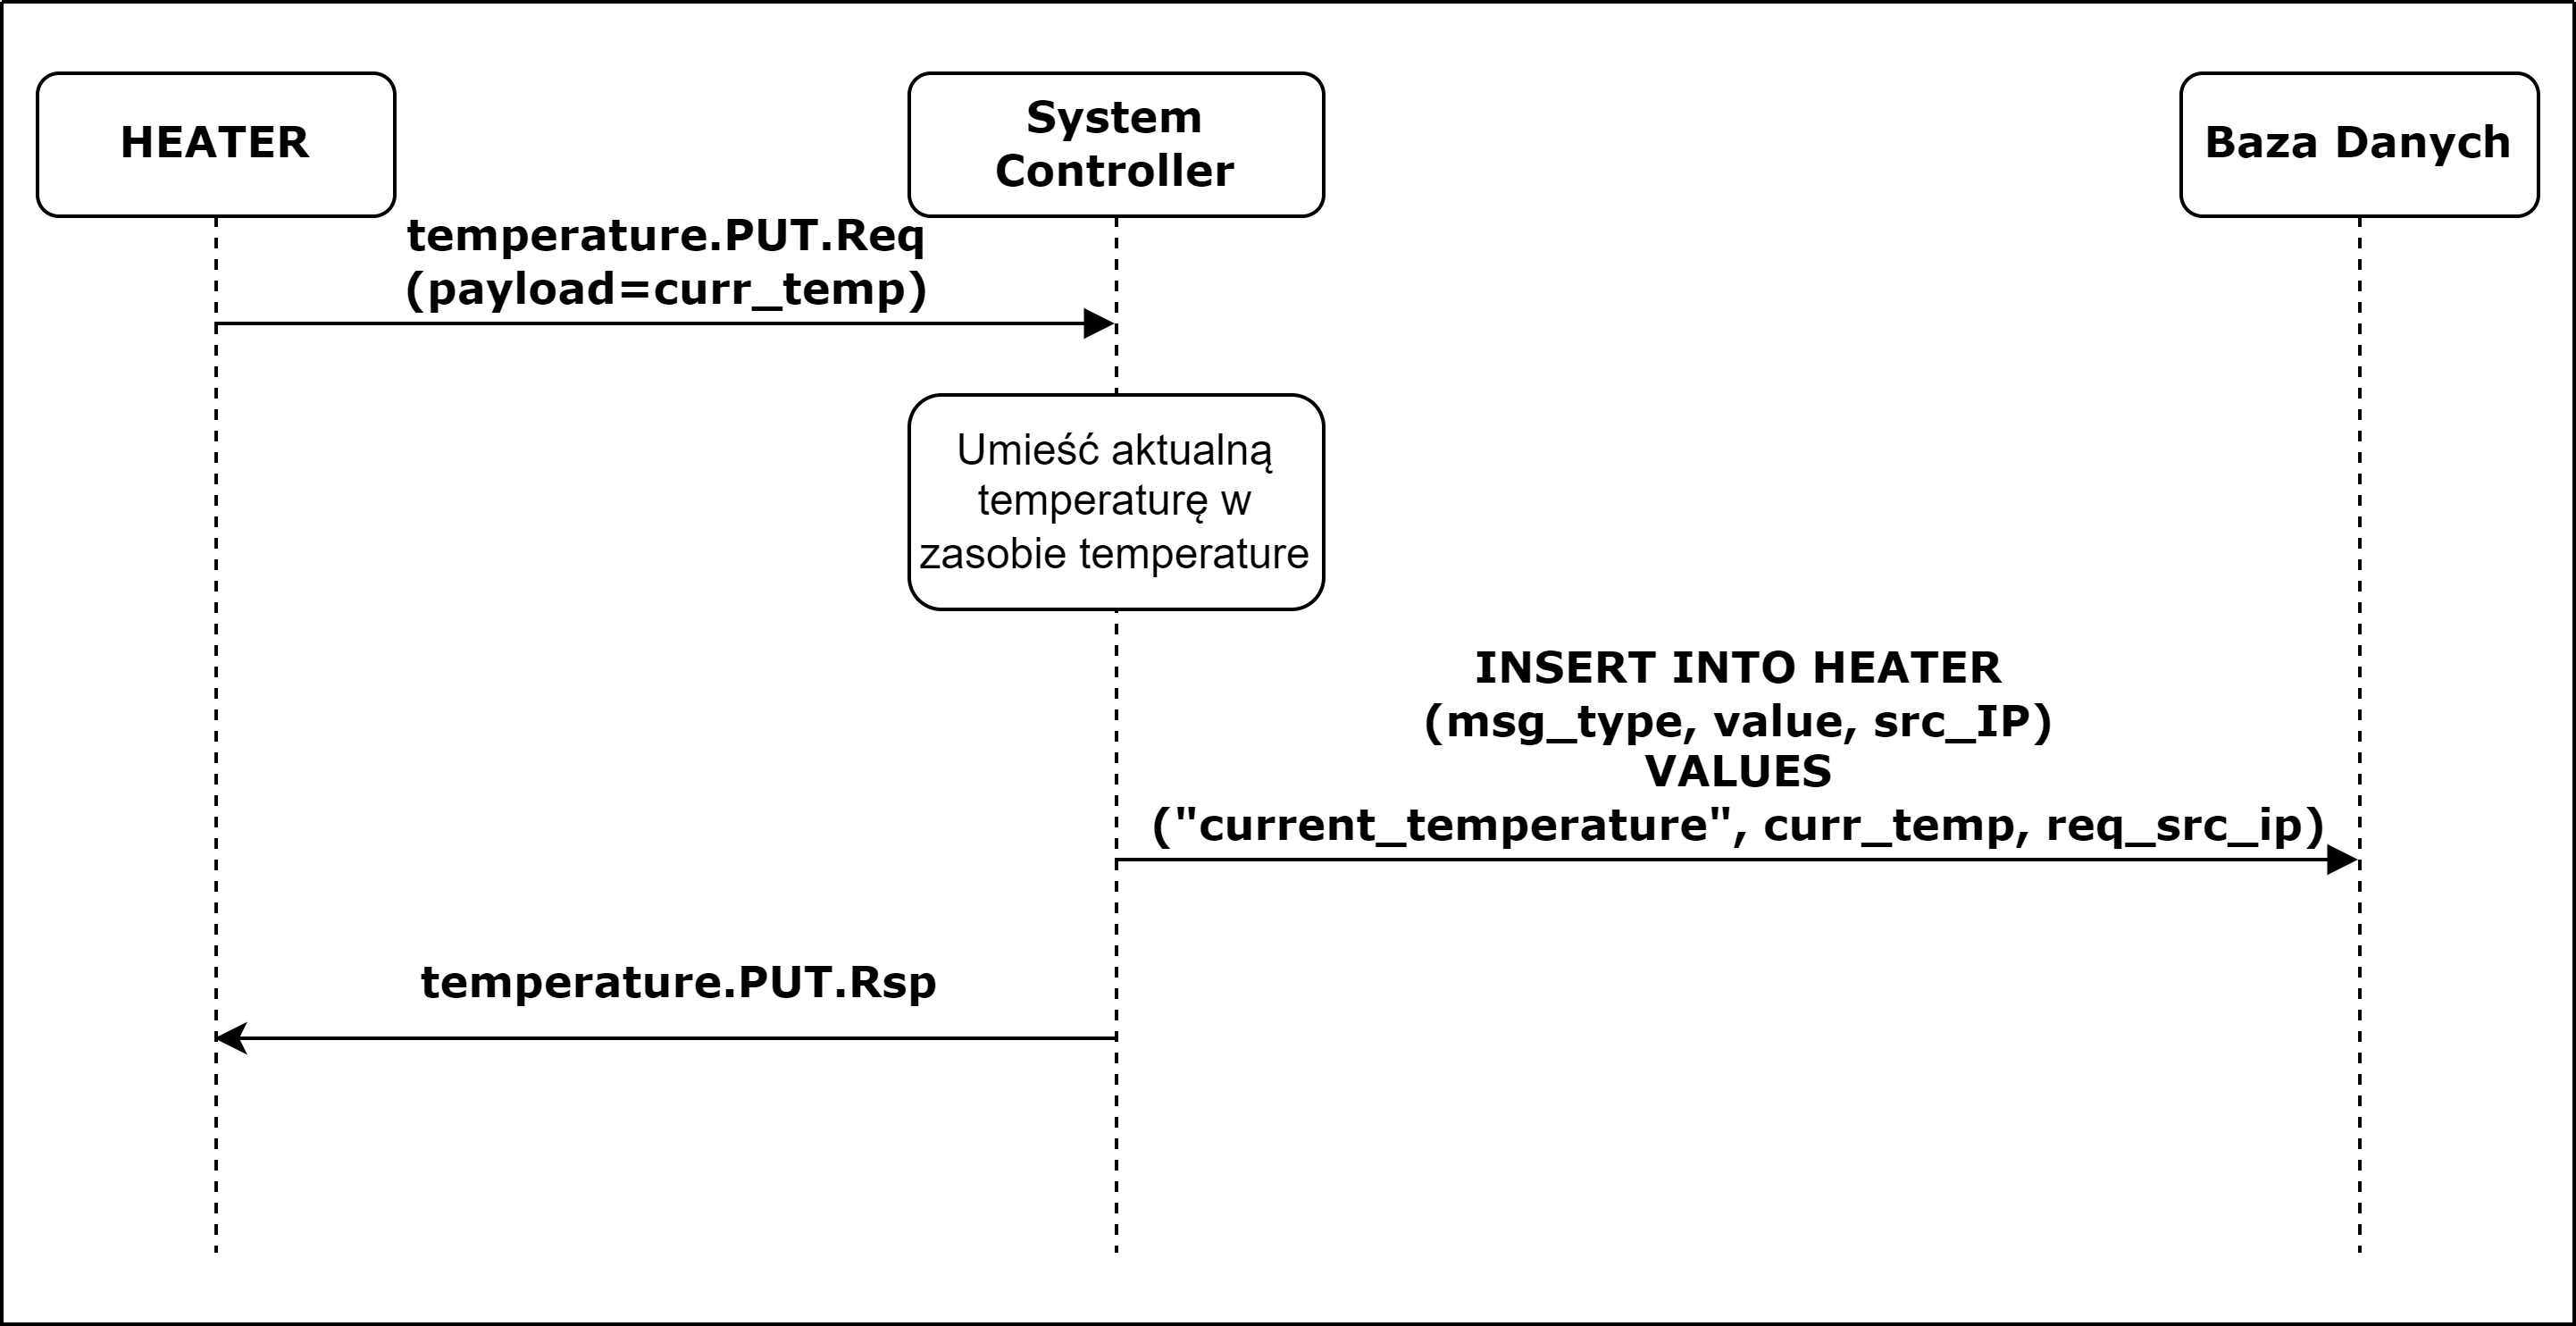
\includegraphics[width=0.8\linewidth]{graphics/sequence-diagrams/heater-measure-seq.png}
                \caption{Diagram sekwencji pomiaru temperatury.}
                \label{fig:seq-heater-measure}
            \end{figure}

            Kolejnymi krokami pomiaru temperatury w fazie pomiaru są:
            \begin{enumerate}
                \item Urządzenie HEATER wysyła zapytanie o umieszczenie temperatury w zasobie \textit{temperature} do System Controllera, w którym umieszcza zmierzoną wartość temperatury.
                \item System Controller umieszcza otrzymaną wartość temperatury w zasobach serwera.
                \item System Controller loguje informację o przetworzonym zapytaniu, umieszczając otrzymaną wartość temperatury w tabeli HEATER Bazy Danych.
                \item System Controller w ramach potwierdzenia otrzymania zapytania, odpowiada układowy HEATER.
            \end{enumerate}

            Na Rysunku \ref{fig:seq-dimmer-measure} zilustrowano przepływ wiadomości między komponentami systemu w fazie pomiaru natężenia oświetlenia.

            \begin{figure}[H]
                \centering
                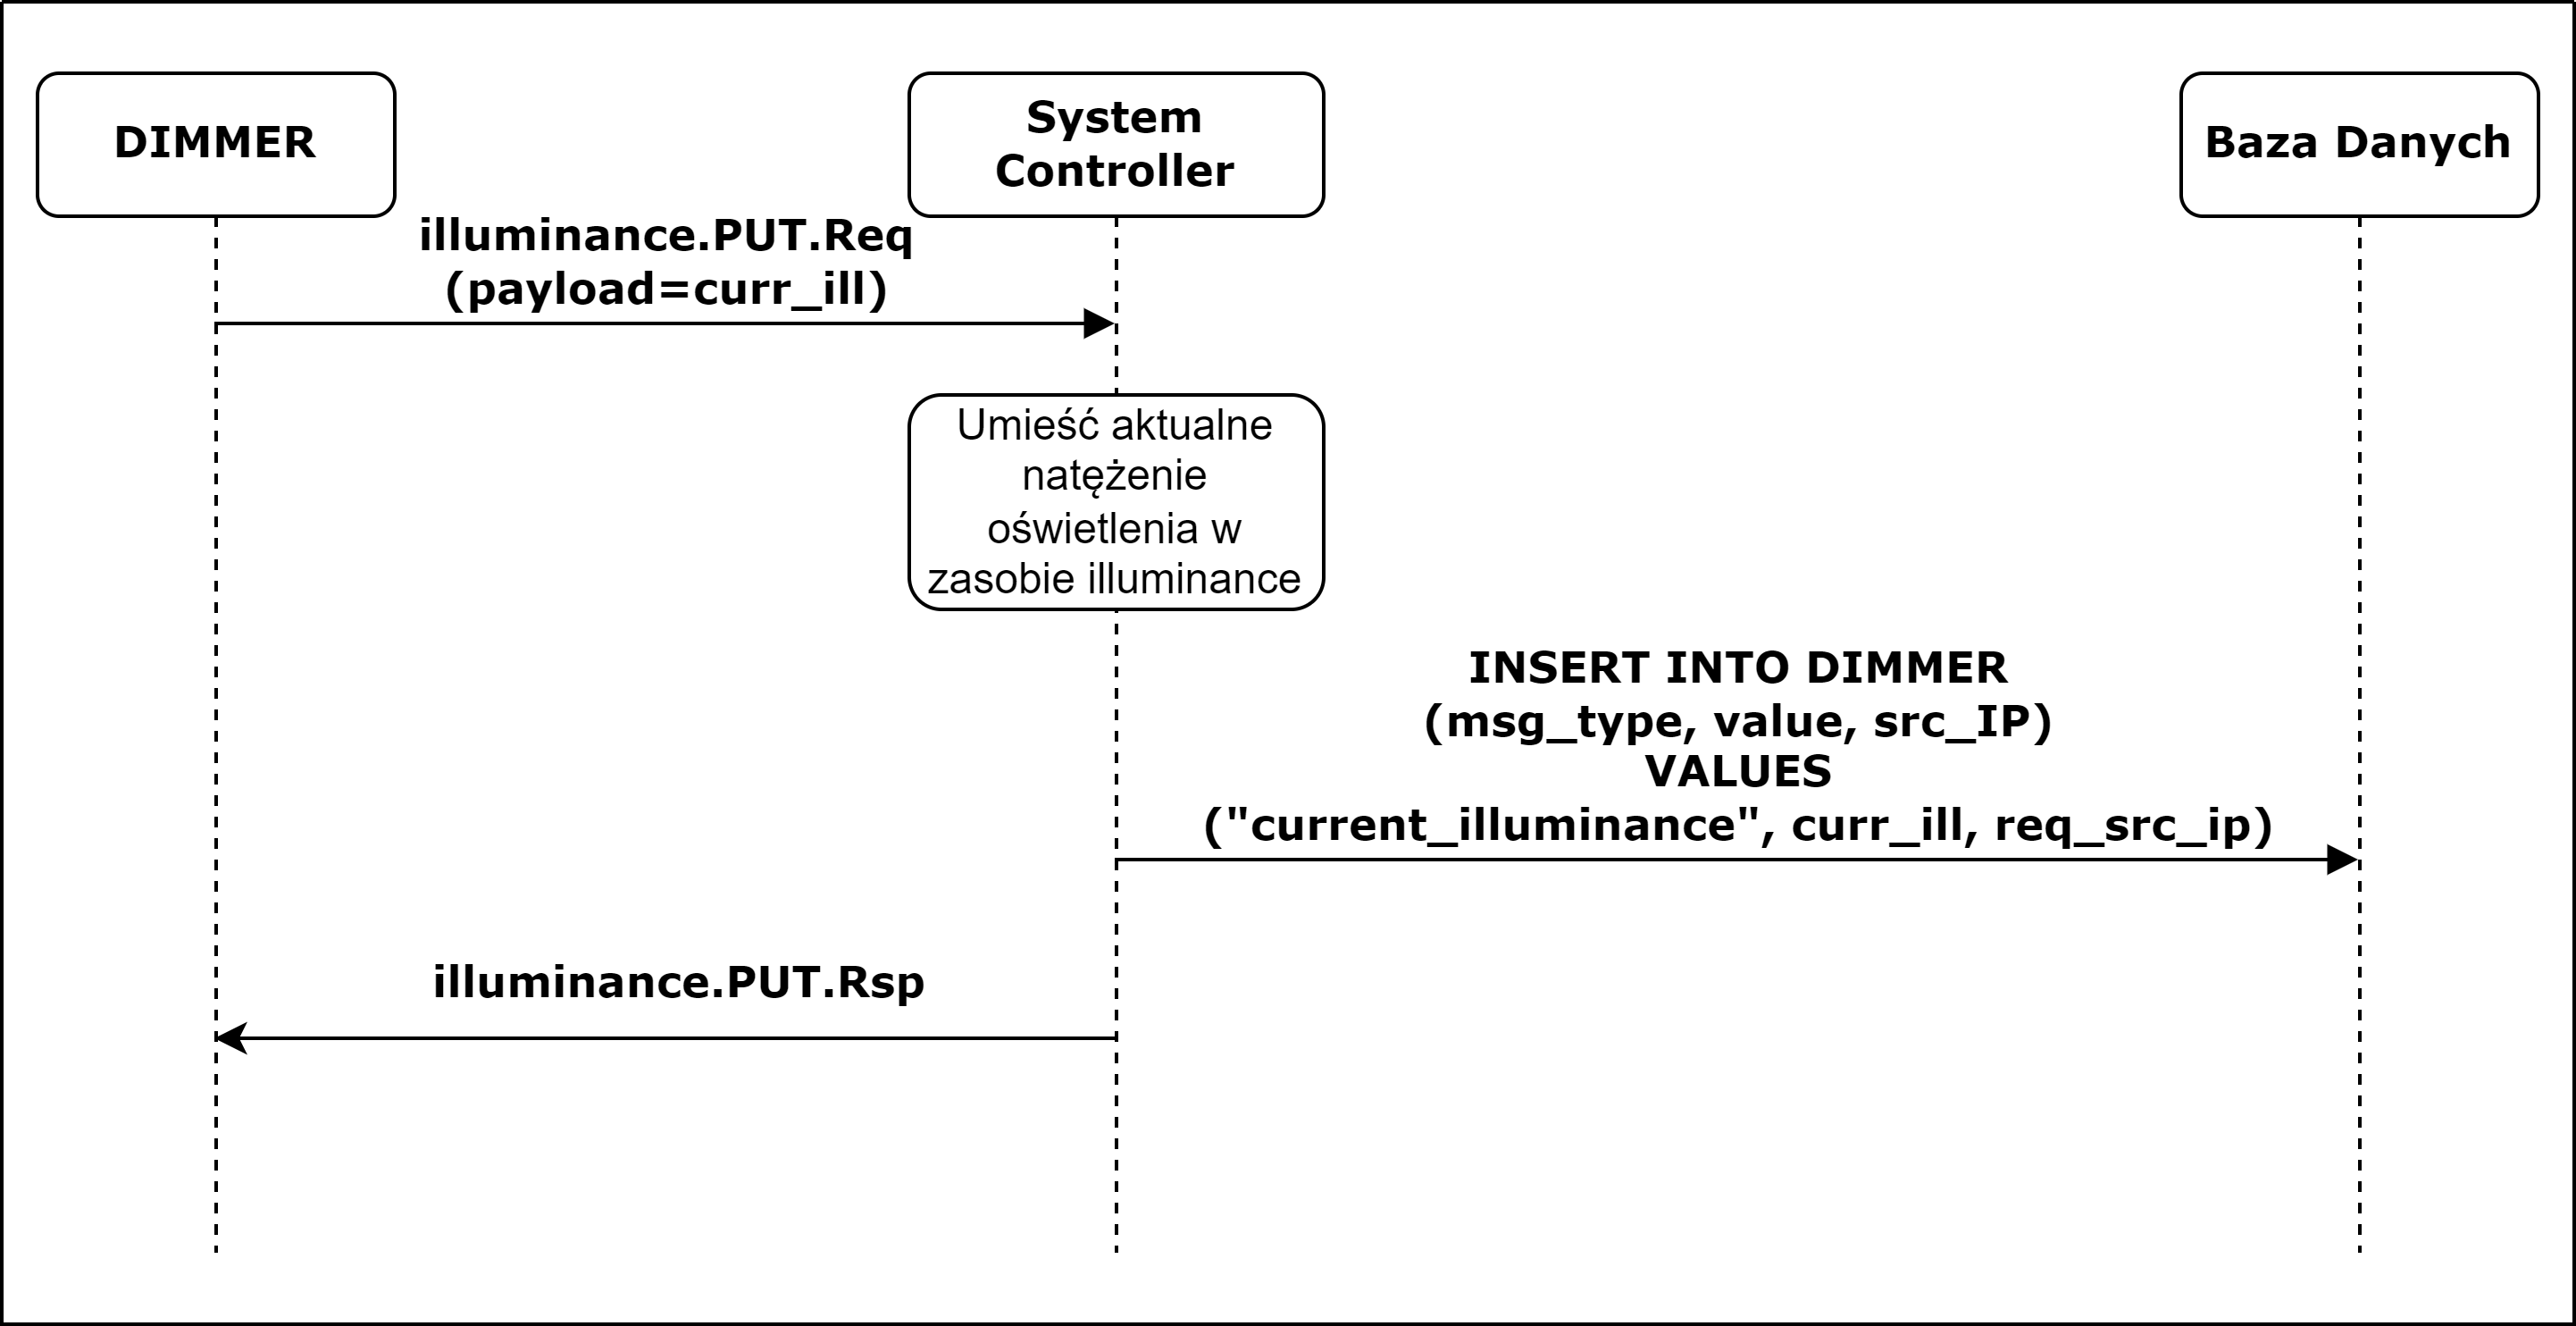
\includegraphics[width=0.8\linewidth]{graphics/sequence-diagrams/dimmer-measure-seq.png}
                \caption{Diagram sekwencji pomiaru natężenia oświetlenia.}
                \label{fig:seq-dimmer-measure}
            \end{figure}

            Kolejnymi krokami pomiaru natężenia oświetlenia w fazie pomiaru są:
            \begin{enumerate}
                \item Urządzenie DIMMER wysyła zapytanie o umieszczenie natężenia oświetlenia w zasobie \textit{illuminance} do System Controllera, w którym umieszcza zmierzoną wartość natężenia oświetlenia.
                \item System Controller umieszcza otrzymaną wartość natężenia oświetlenia w zasobach serwera.
                \item System Controller loguje informację o przetworzonym zapytaniu, umieszczając otrzymaną wartość natężenia oświetlenia w tabeli DIMMER Bazy Danych.
                \item System Controller w ramach potwierdzenia otrzymania zapytania, odpowiada układowy HEATER.
            \end{enumerate}


        \subsubsection{Regulacja}

            Na Rysunku \ref{fig:seq-heater-regulate} zilustrowano przepływ wiadomości między komponentami systemu w fazie regulacji temperatury.

            \begin{figure}[H]
                \centering
                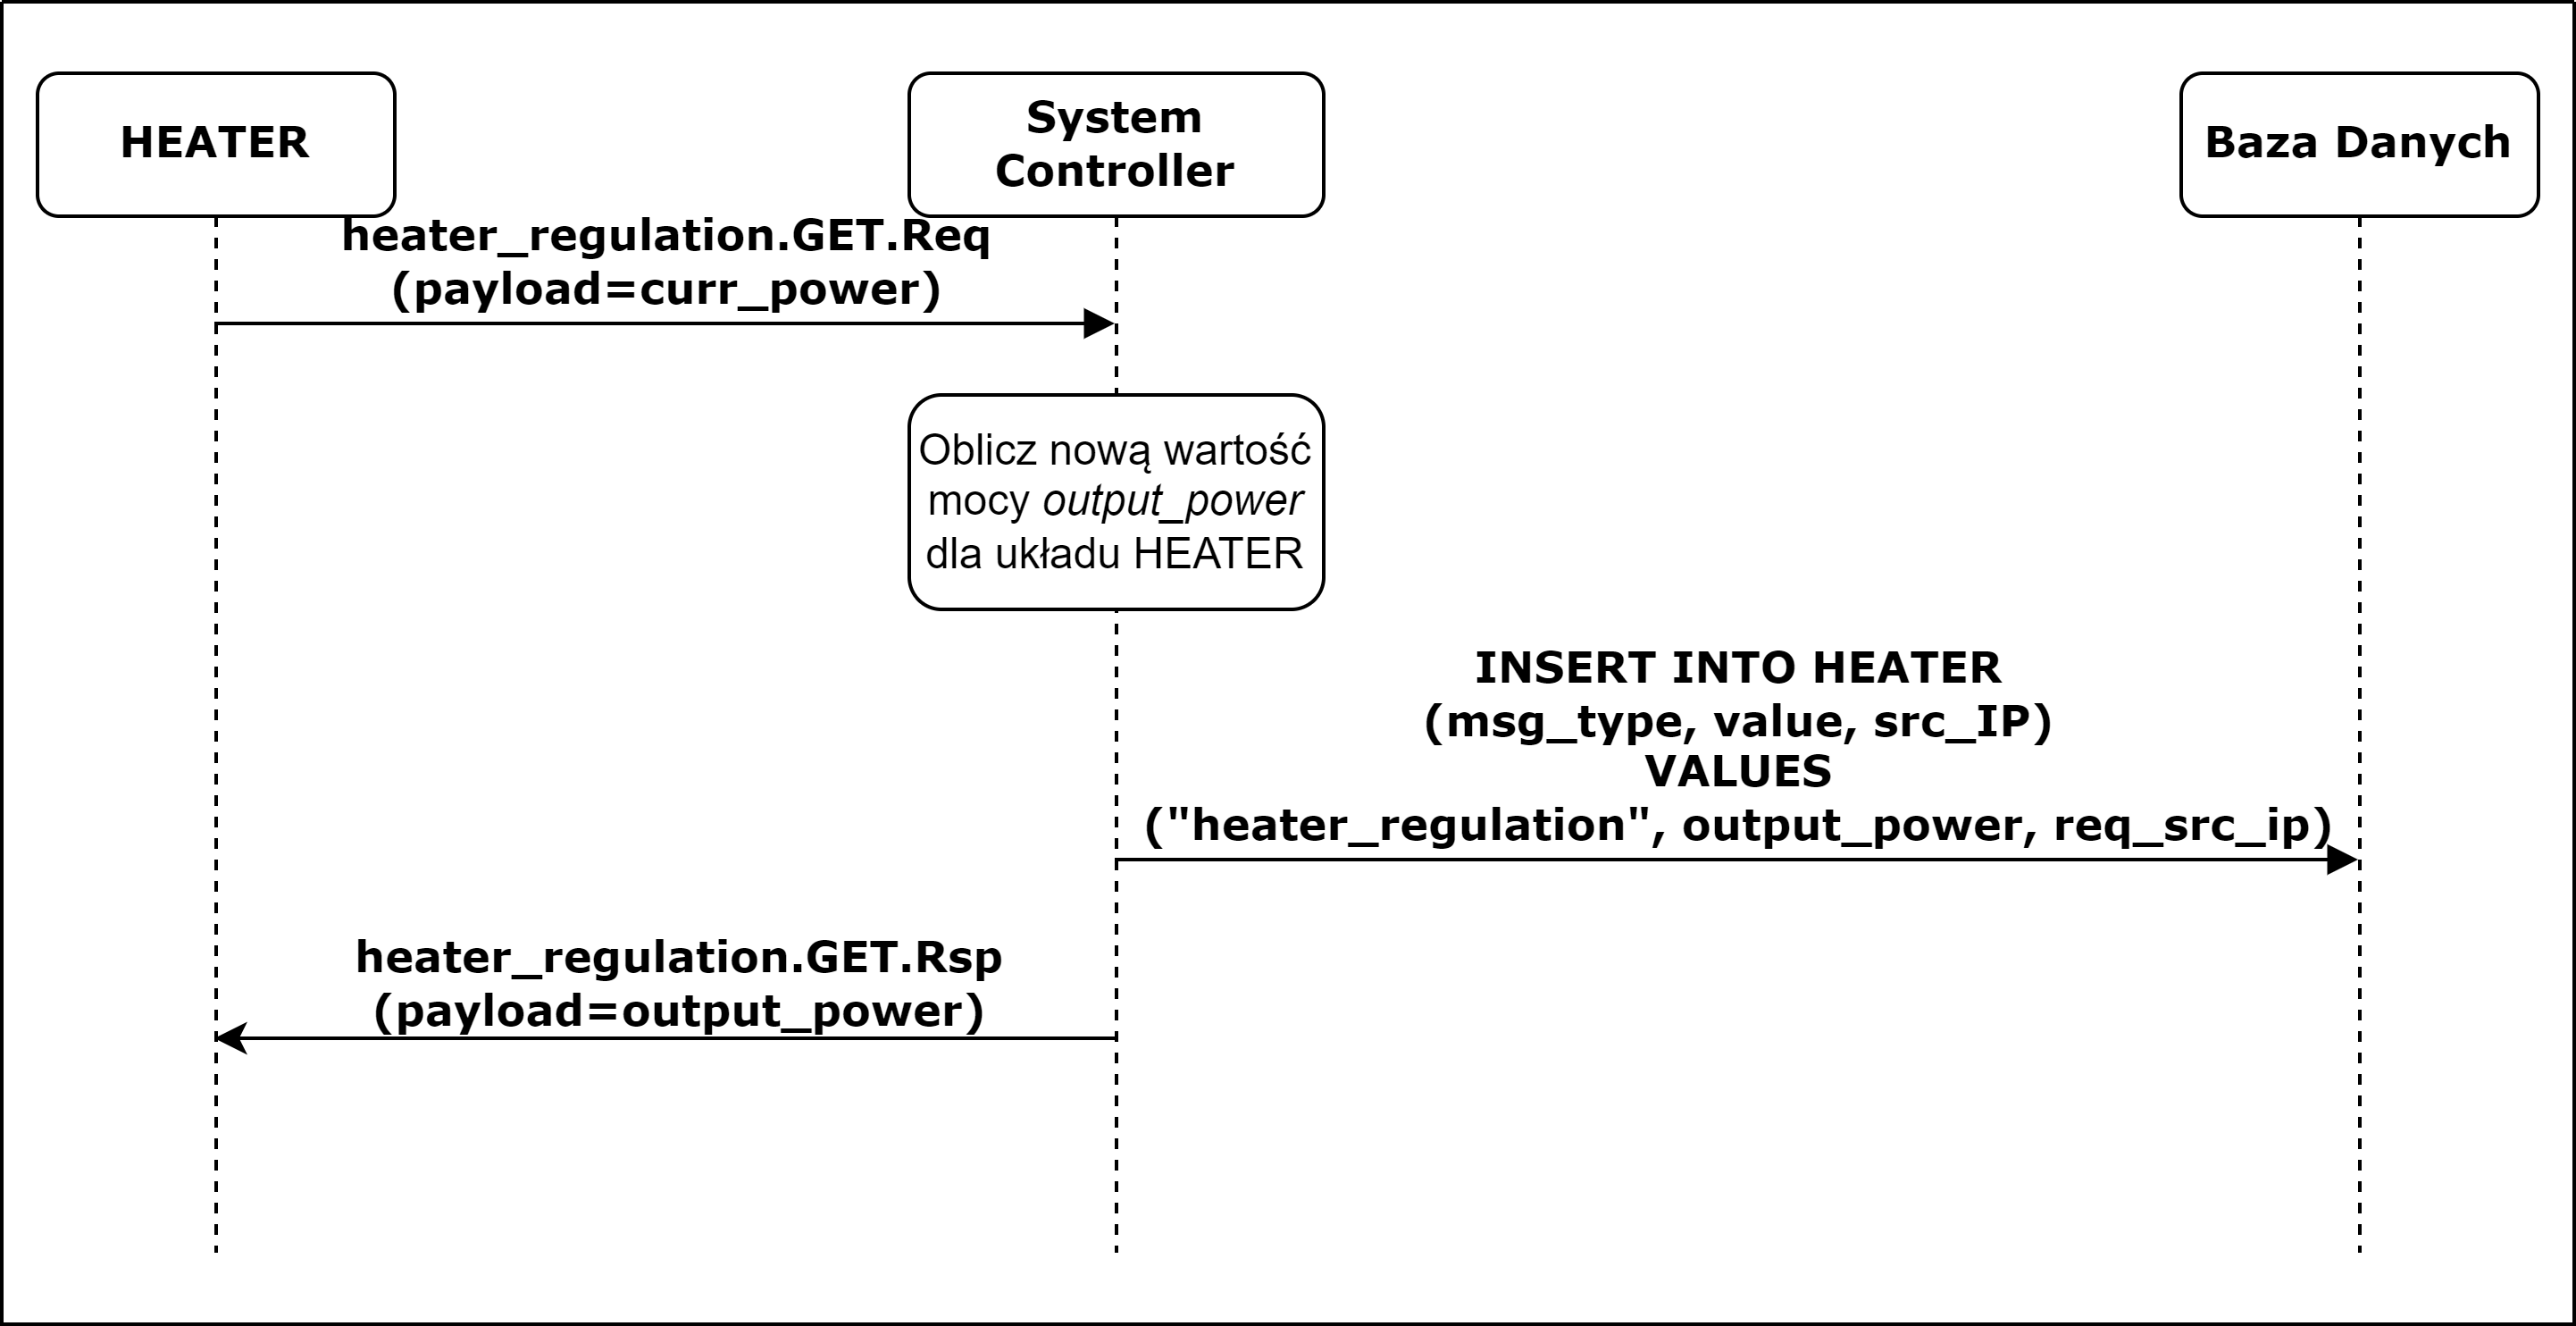
\includegraphics[width=0.8\linewidth]{graphics/sequence-diagrams/heater-regulate-seq.png}
                \caption{Diagram sekwencji regulacji temperatury.}
                \label{fig:seq-heater-regulate}
            \end{figure}

            \begin{figure}[H]
                \centering
                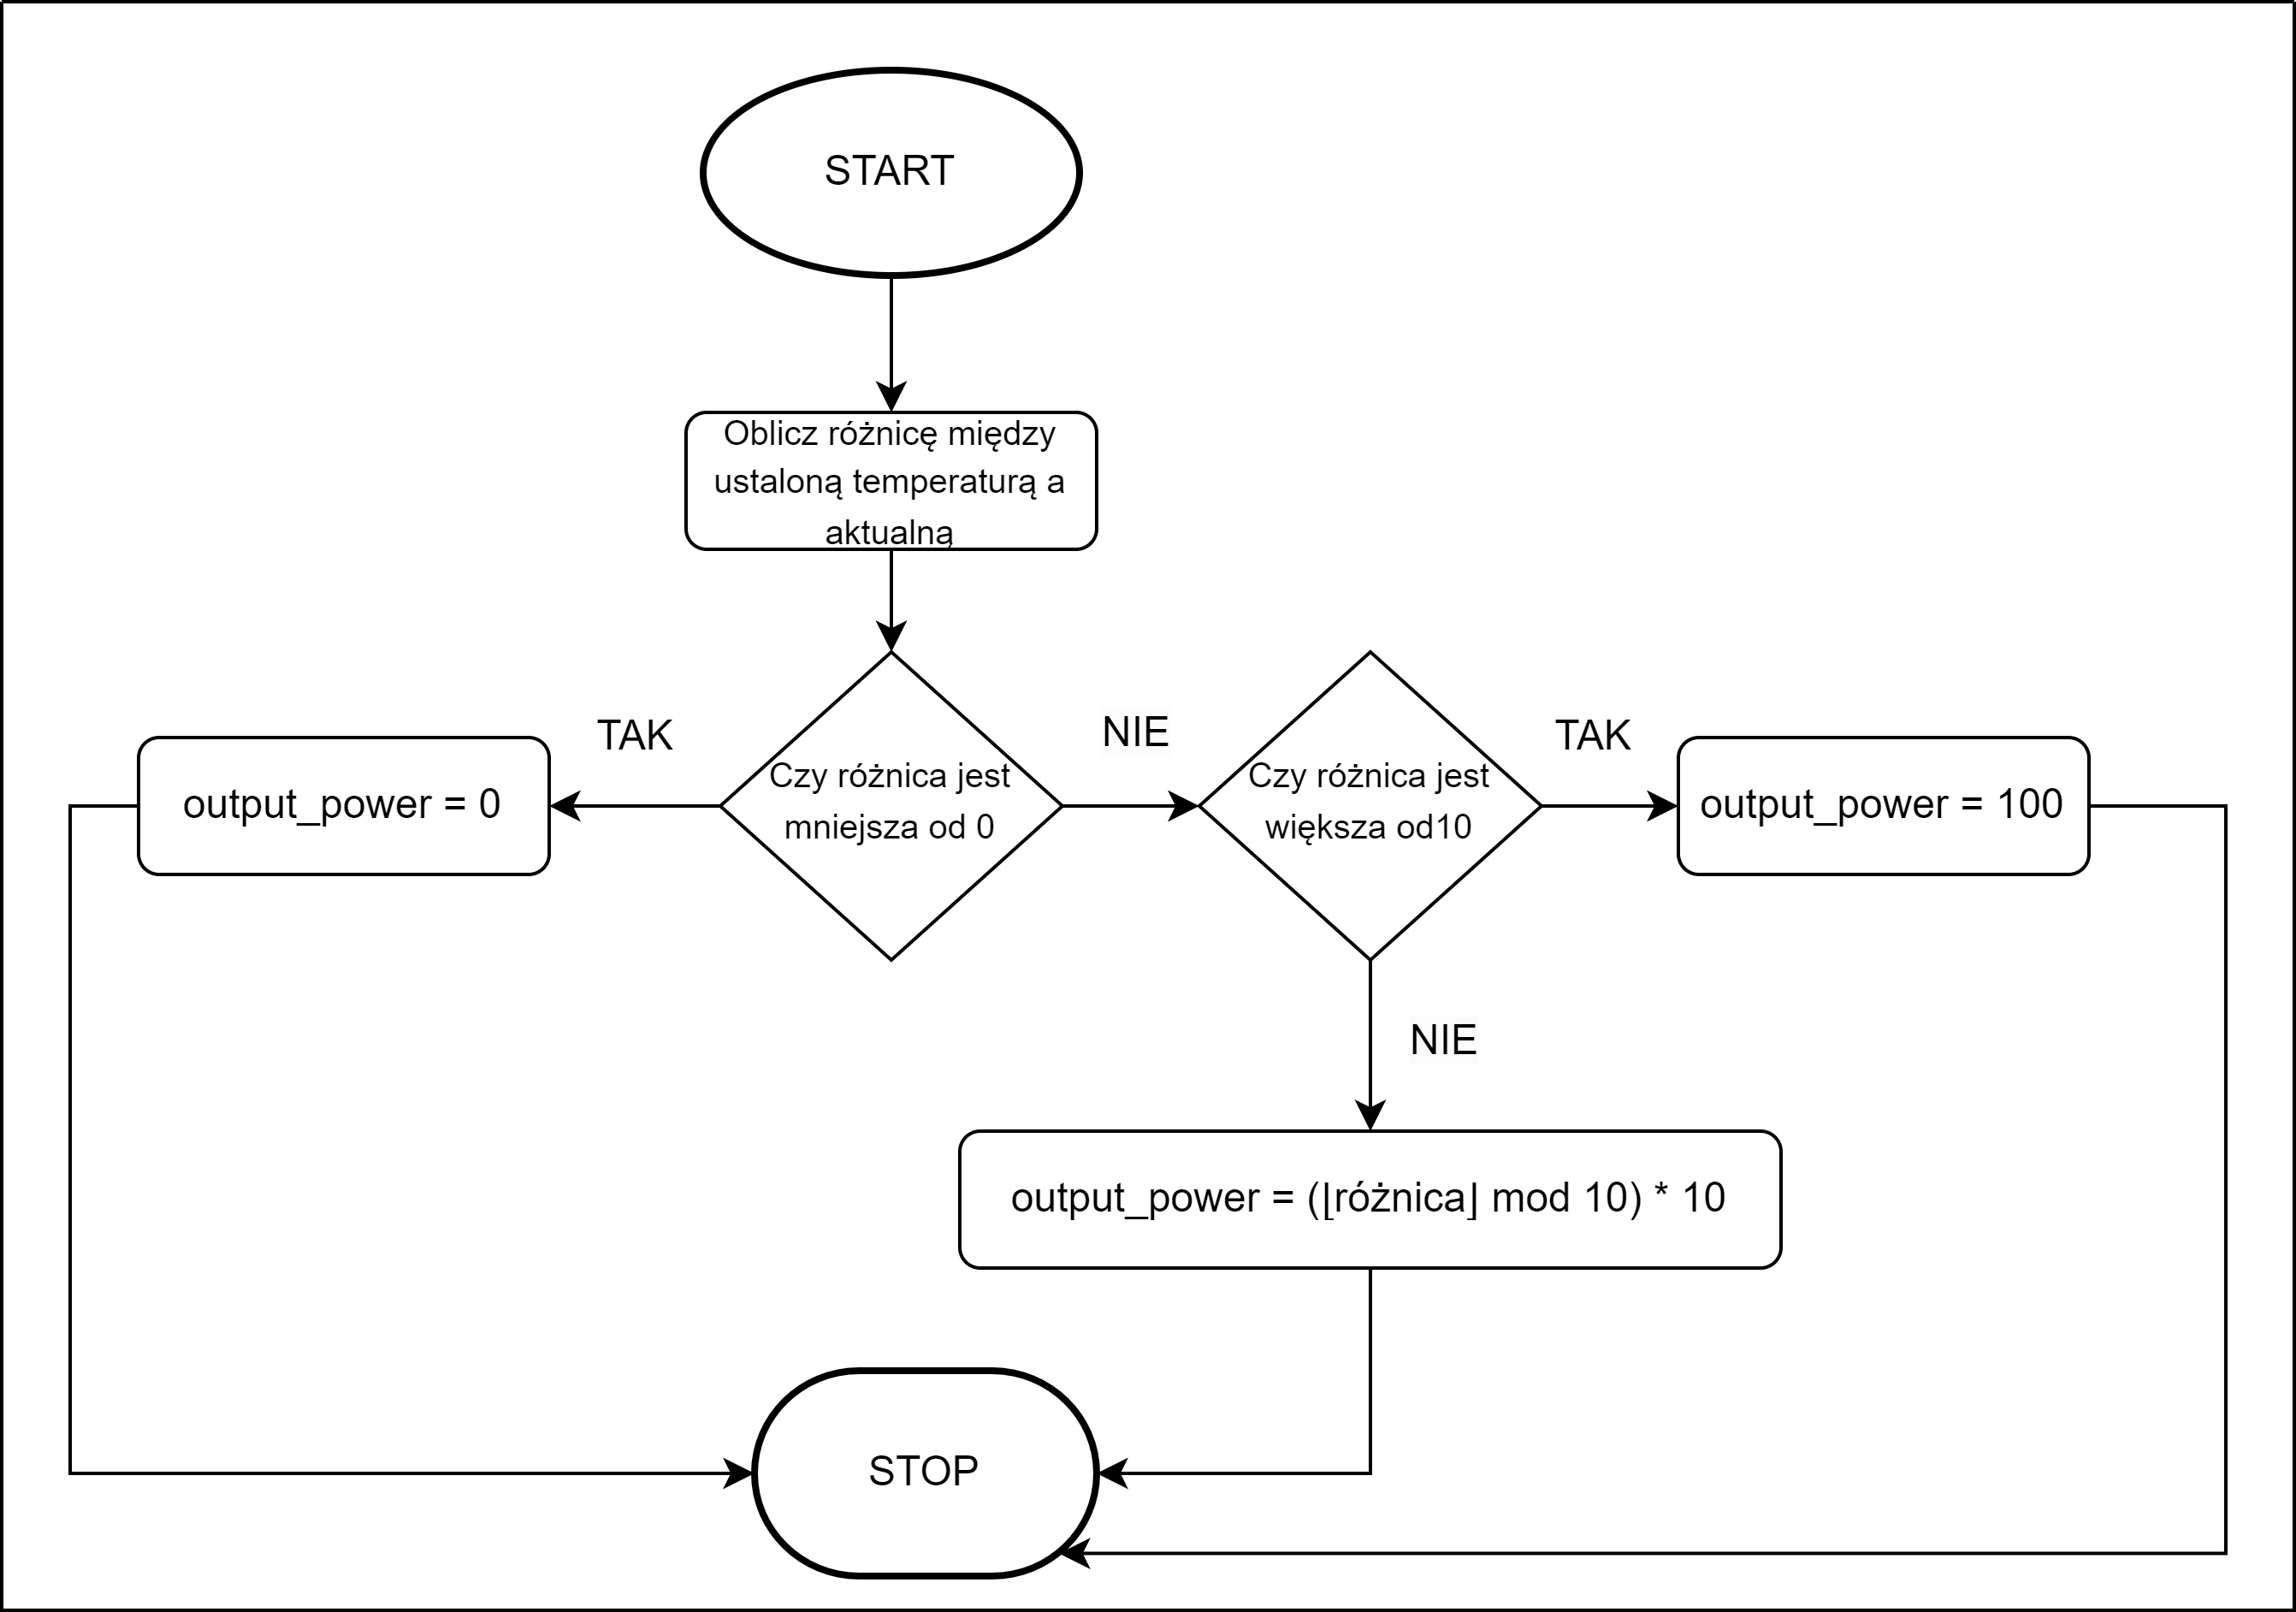
\includegraphics[width=0.8\linewidth]{graphics/heater-block-diagram.png}
                \caption{Algorytm obliczania parametru mocy dla układu HEATER.}
                \label{fig:seq-heater-algo}
            \end{figure}

            Kolejnymi krokami regulacji temperatury w fazie regulacji są:
            \begin{enumerate}
                \item Urządzenie HEATER wysyła zapytanie o otrzymanie nowego parametru mocy w zasobie \\ \textit{heater\_regulation} do System Controllera, w którym umieszcza aktualną wartość parametru mocy.
                \item System Controller oblicza nową wartość \textit{output\_power} na podstawie wartości aktualnej temperatury, umieszczonej w zasobie \textit{temperature} oraz poprzedniej wartości parametru mocy \textit{curr\_power}, zgodnie z algorytmem przedstawionym na Rysunku \ref{fig:seq-heater-algo}.
                \item System Controller loguje informację o przetworzonym zapytaniu, umieszczając obliczoną wartość \\ \textit{output\_power} w tabeli HEATER Bazy Danych.
                \item System Controller odpowiada układowy HEATER, dostarczając nową wartość parametru mocy \\ \textit{output\_power}.
            \end{enumerate}

            Na Rysunku \ref{fig:seq-dimmer-regulate} zilustrowano przepływ wiadomości między komponentami systemu w fazie regulacji natężenia oświetlenia.

            \begin{figure}[H]
                \centering
                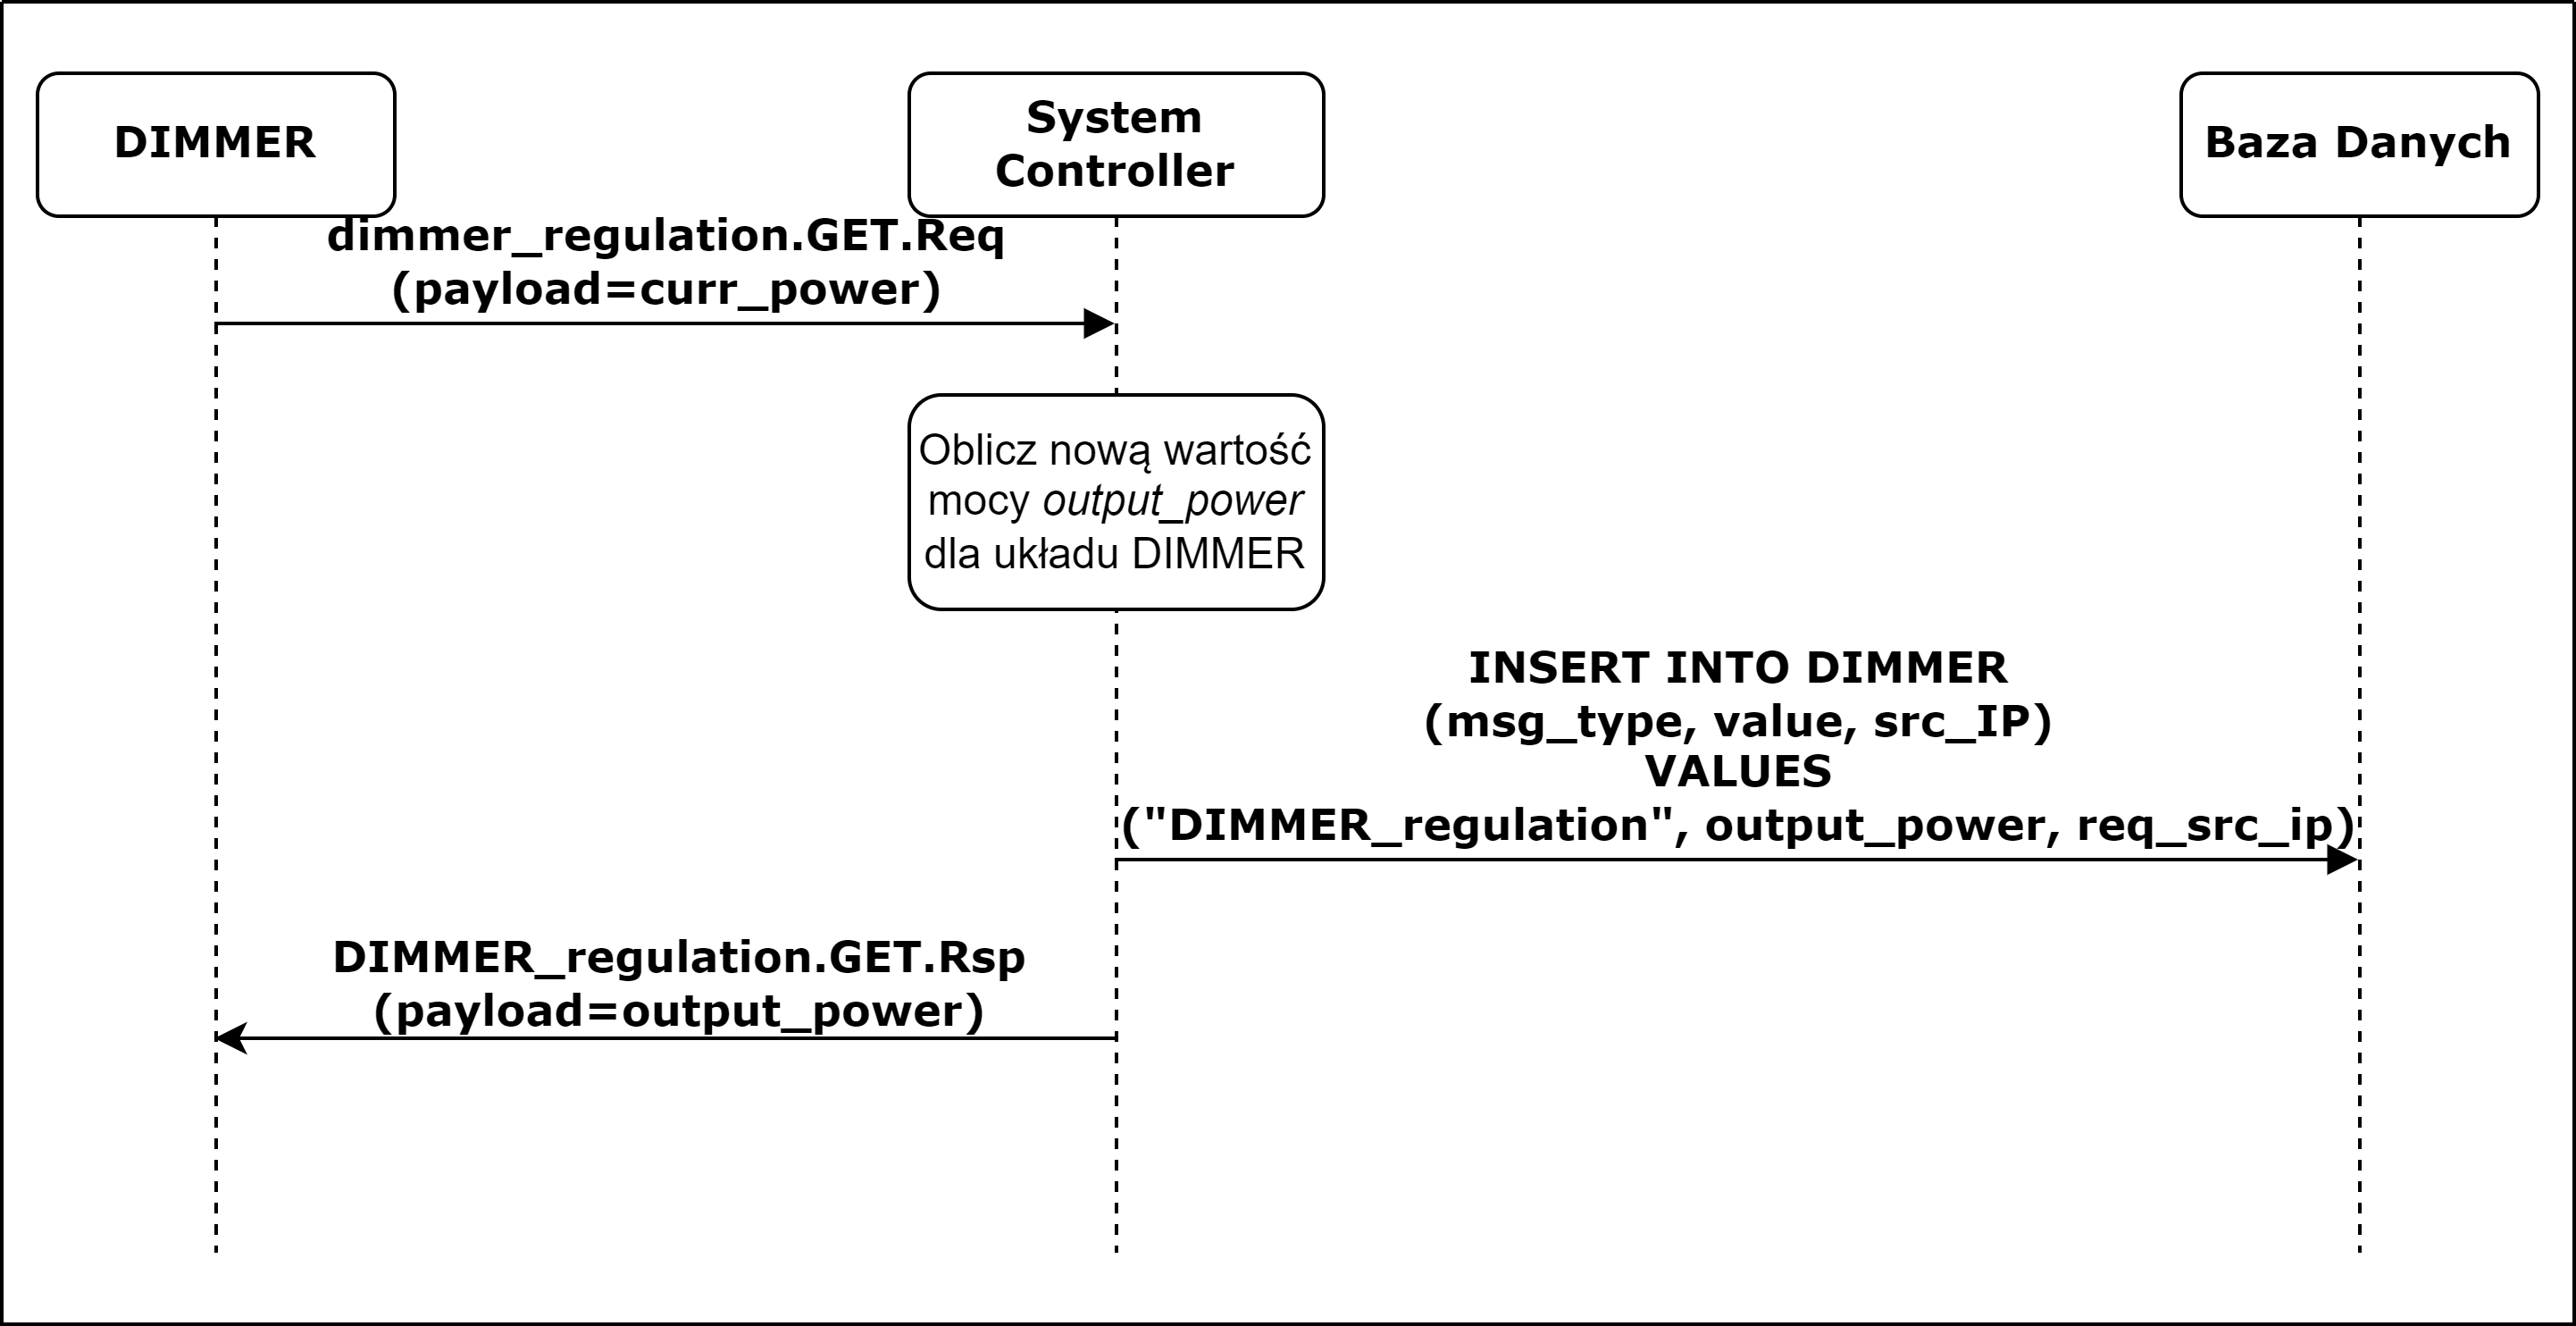
\includegraphics[width=0.8\linewidth]{graphics/sequence-diagrams/dimmer-regulate-seq.png}
                \caption{Diagram sekwencji regulacji natężenia oświetlenia.}
                \label{fig:seq-dimmer-regulate}
            \end{figure}

            \begin{figure}[H]
                \centering
                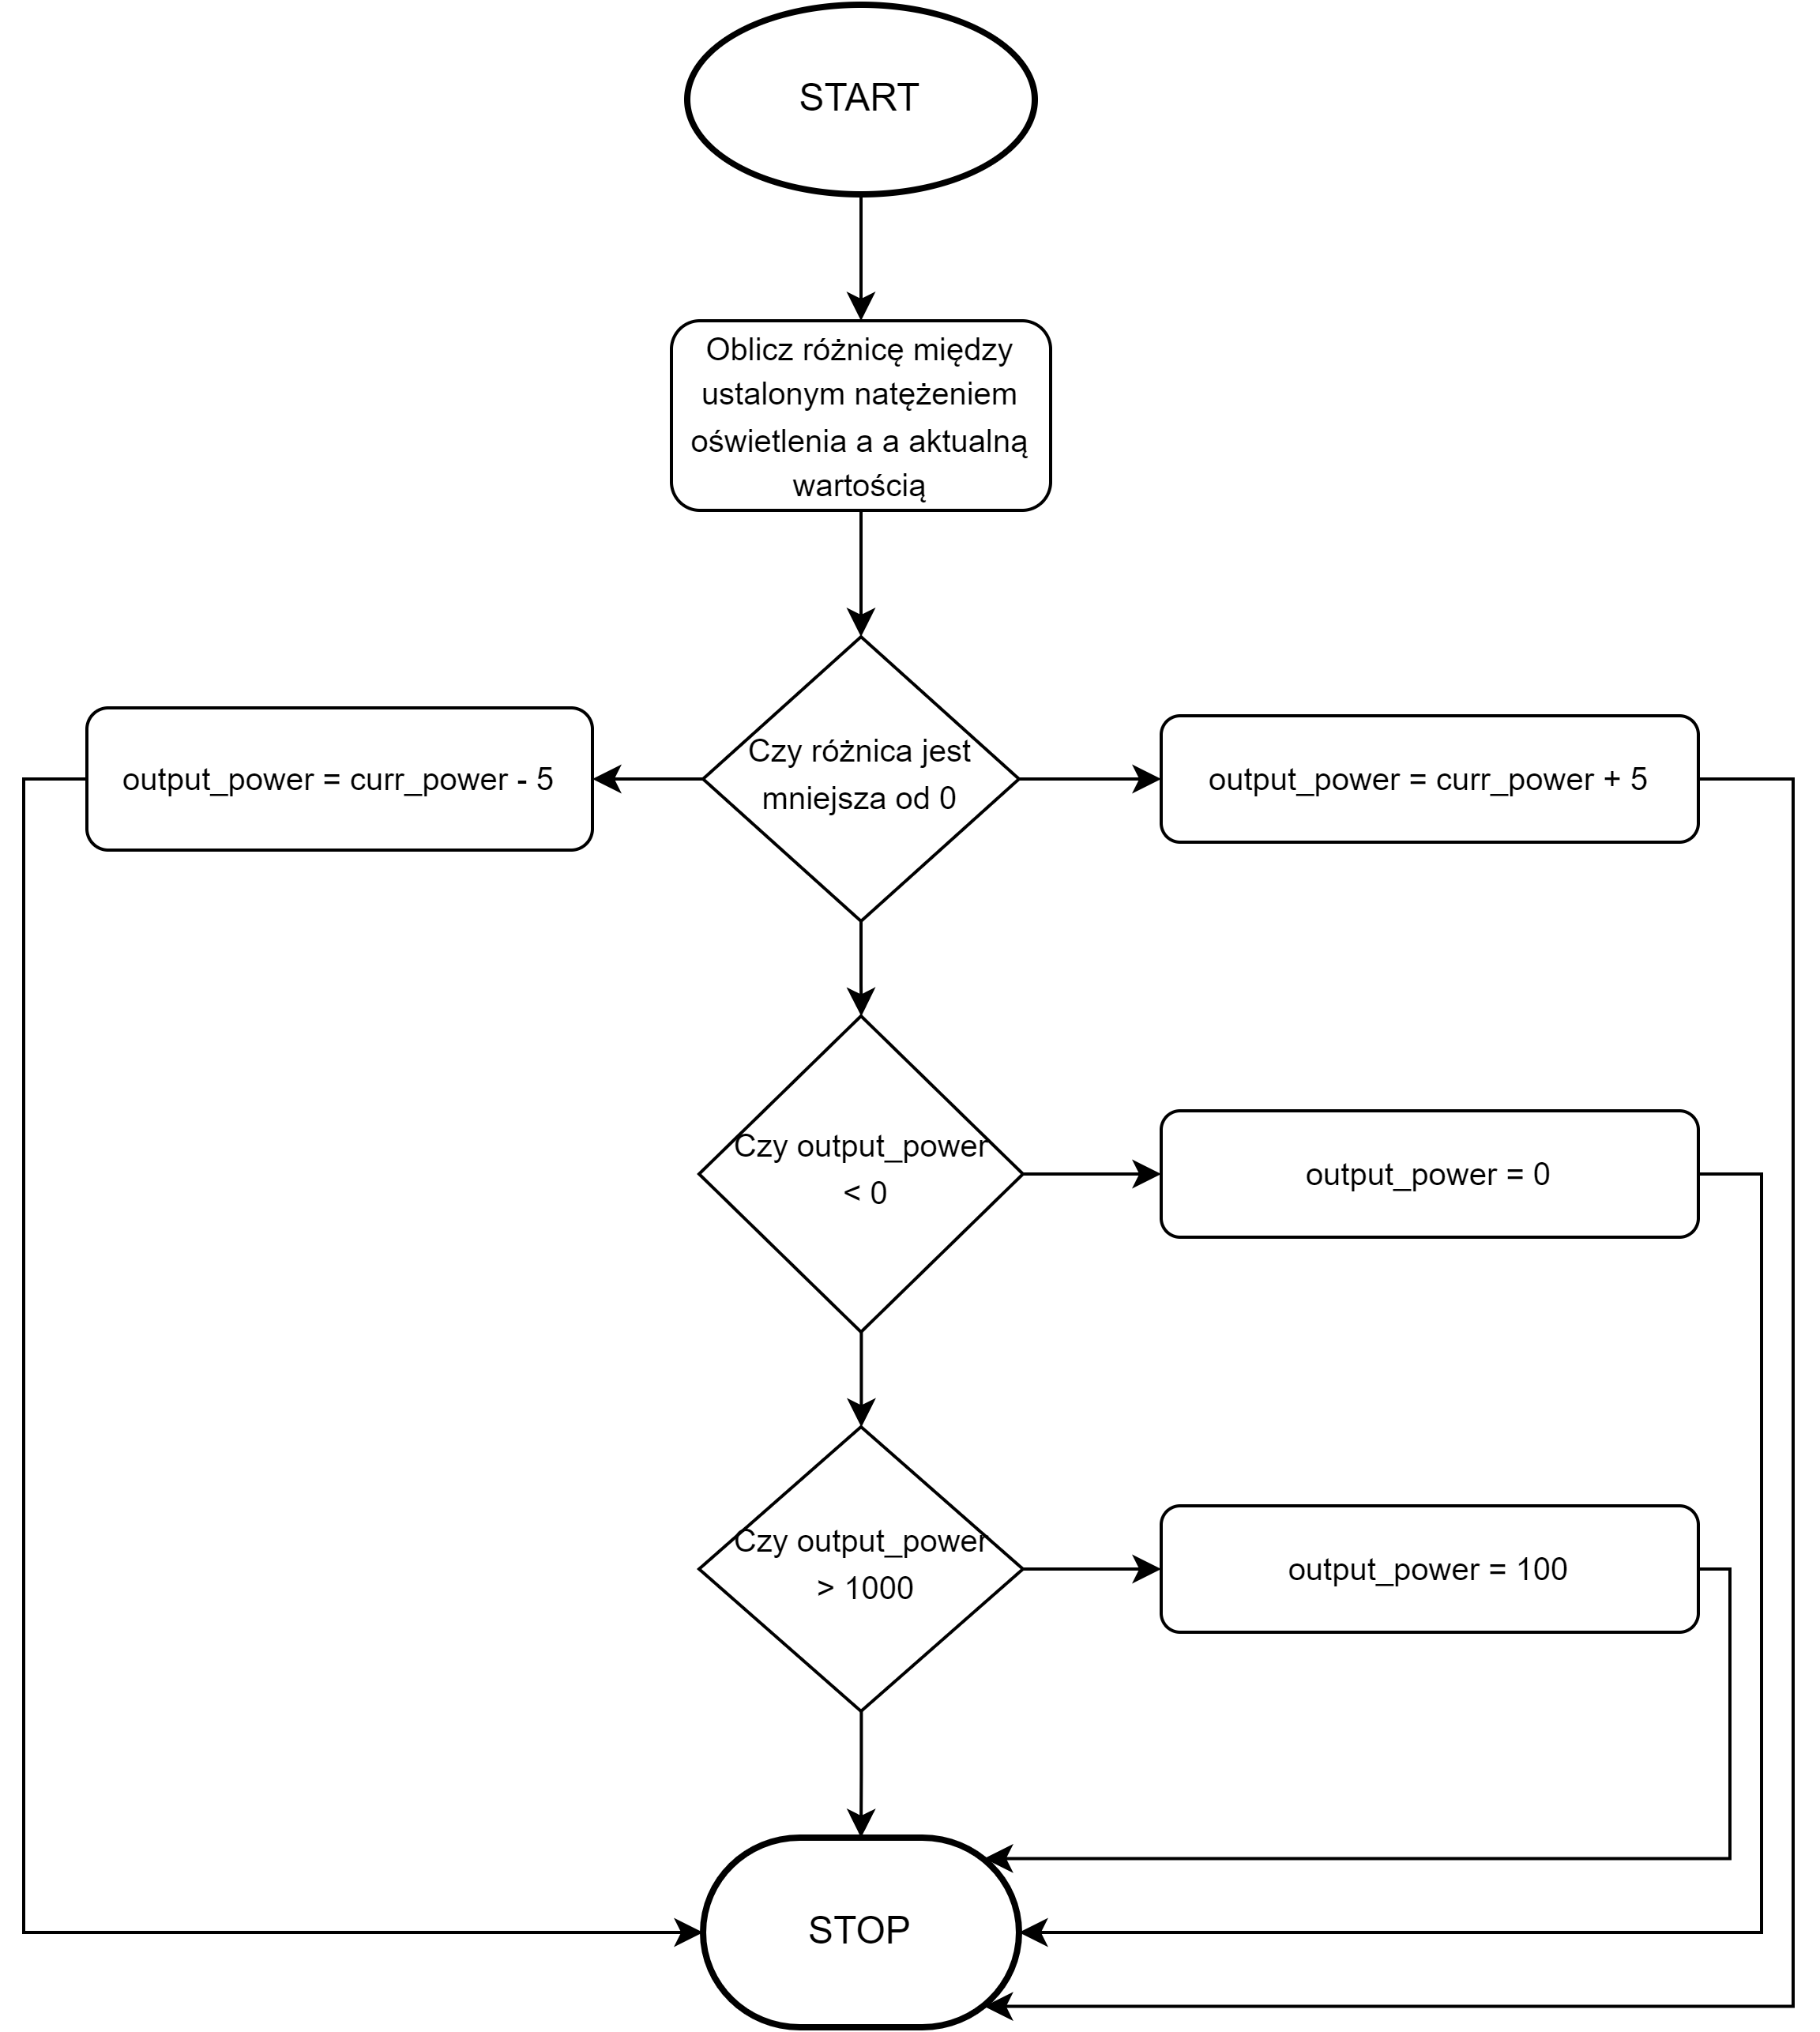
\includegraphics[width=0.8\linewidth]{graphics/dimmer-block-diagram.png}
                \caption{Algorytm obliczania parametru mocy dla układu DIMMER.}
                \label{fig:seq-dimmer-algo}
            \end{figure}

            Kolejnymi krokami regulacji temperatury w fazie regulacji są:
            \begin{enumerate}
                \item Urządzenie DIMMER wysyła zapytanie o otrzymanie nowego parametru mocy w zasobie \\ \textit{dimmer\_regulation} do System Controllera, w którym umieszcza aktualną wartość parametru mocy.
                \item System Controller oblicza nową wartość \textit{output\_power} na podstawie wartości aktualnego natężenia oświetlenia, umieszczonego w zasobie \textit{illuminance} oraz poprzedniej wartości parametru mocy \textit{curr\_power}, zgodnie z algorytmem przedstawionym na Rysunku \ref{fig:seq-dimmer-algo}.
                \item System Controller loguje informację o przetworzonym zapytaniu, umieszczając obliczoną wartość \\ \textit{output\_power} w tabeli DIMMER Bazy Danych.
                \item System Controller odpowiada układowy DIMMER, dostarczając nową wartość parametru mocy \\ \textit{output\_power}.
            \end{enumerate}

